\documentclass[a4paper,openright,12pt]{report}
\usepackage[spanish]{babel}
\usepackage[utf8]{inputenc}
%\usepackage{cite}
\usepackage{graphicx}
\usepackage{pdfpages}
\usepackage{fancyhdr}
\usepackage[ruled,vlined,linesnumbered]{algorithm2e}
\usepackage{url}
\makeatletter%para cortar url largos en varias lineas
\g@addto@macro{\UrlBreaks}{\UrlOrds}
\makeatother%%%%

\usepackage{hyperref}
\setcounter{secnumdepth}{3}%hasta subsubsection
\setcounter{tocdepth}{3}
\usepackage{subfigure} % subfiguras
\usepackage{multirow, array} % para las tablas
\usepackage{float} % para usar [H]
\usepackage{verbatim} % comentarios
\usepackage{setspace}
\usepackage{natbib}
\bibliographystyle{unsrtnat}


\hypersetup{
	colorlinks,
	citecolor=black,
	filecolor=black,
	linkcolor=black,
	urlcolor=black
}


\begin{document}
\renewcommand{\listtablename}{Índice de tablas}
\renewcommand{\tablename}{Tabla}


%título

\begin{titlepage}

\AddToShipoutPicture*{\put(0,0){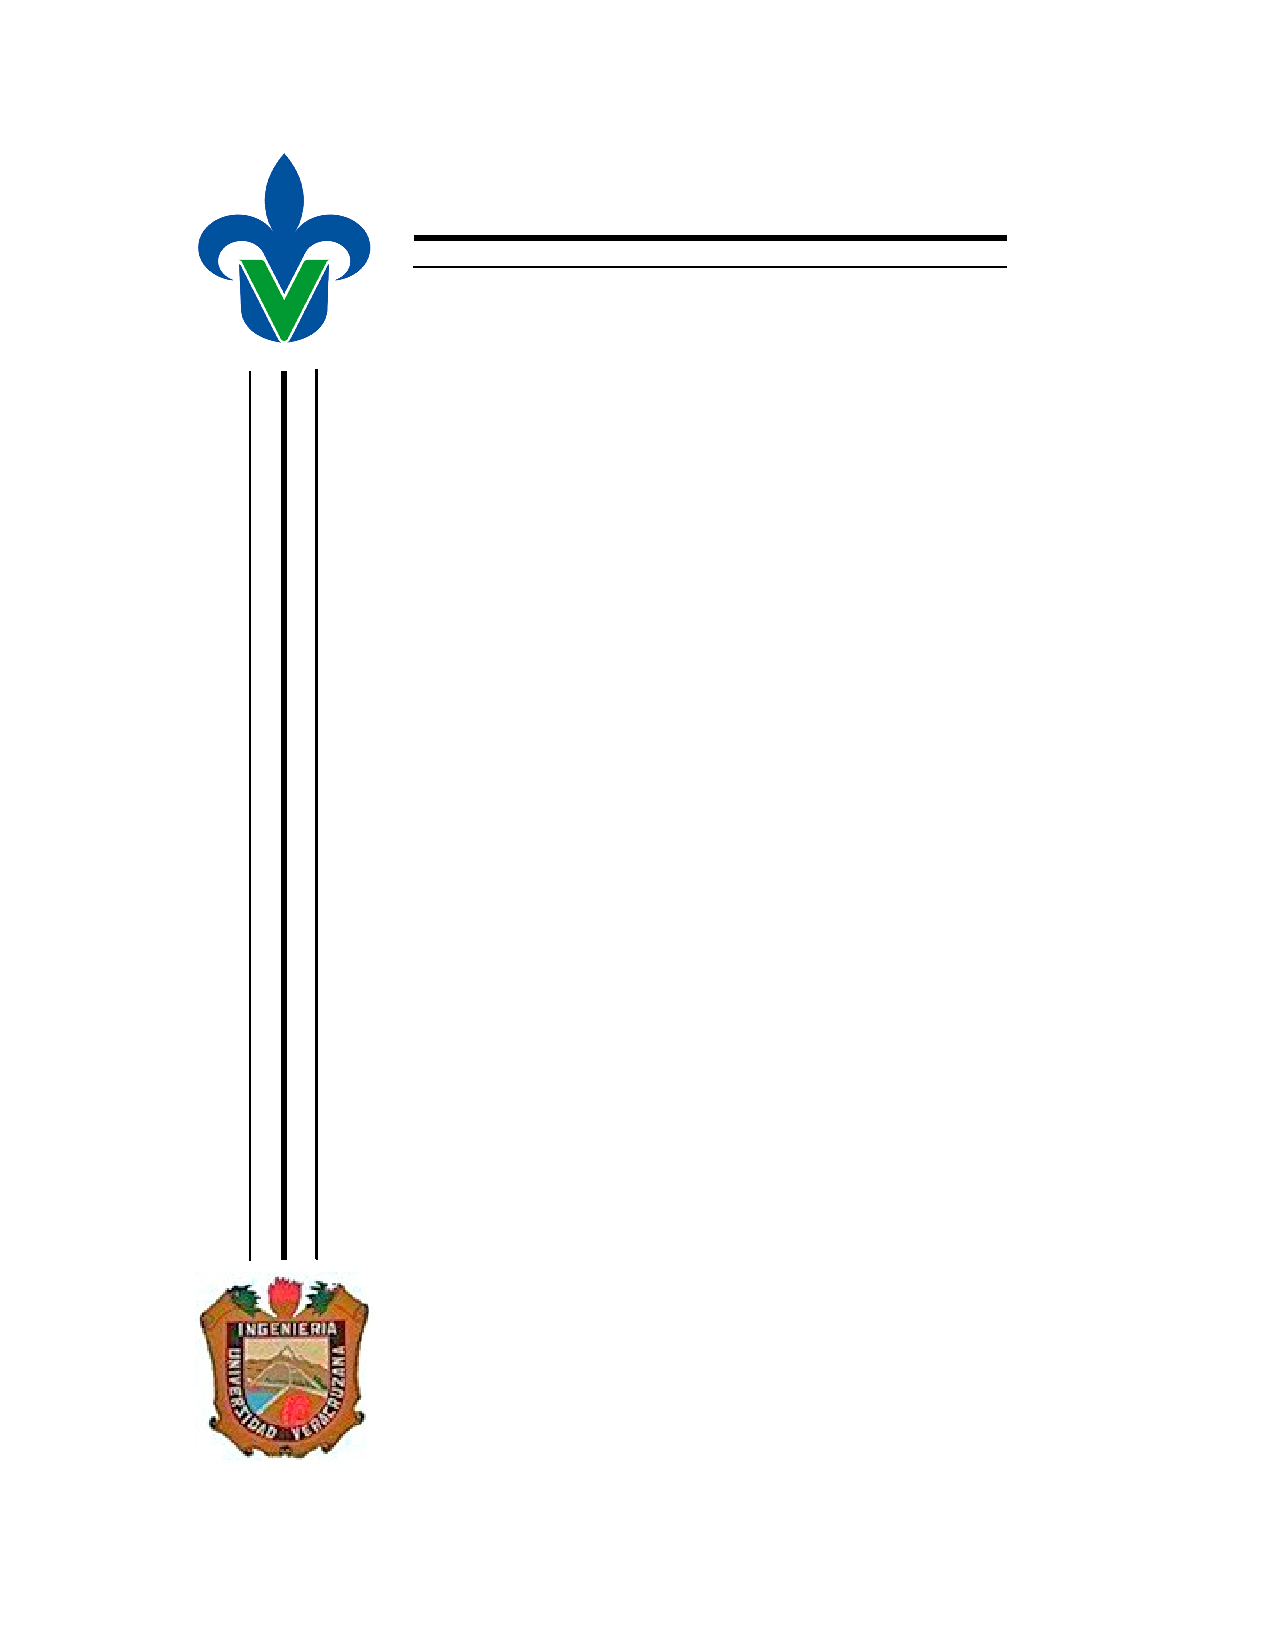
\includegraphics[scale=1]{portada2.pdf}}} % Image background
	
	\begin{minipage}[t][1.75cm][b]{1.15\textwidth}
		\begin{center}
			\begin{Large}
				\textsc{Universidad Veracruzana}
			\end{Large}	
			\\
			\vspace*{0.6cm}
			\textsc{Facultad de Ingeniería}
		\end{center}
	\end{minipage}
\hspace*{3.6cm}
\mbox{	
\begin{minipage}[b][6cm][b]{0.7\textwidth}
	\begin{center}
		\begin{LARGE}
			\textsc{Proyección Adaptativa de un
				escenario 3D basado en la
				perspectiva de una persona}
		\end{LARGE}	
		
	\end{center}
\end{minipage}
	}
	\\
\hspace*{3.6cm}	
	\mbox{	
		\begin{minipage}[b][7.5cm][b]{0.7\textwidth}
			\begin{center}
					\textsc{
						\large Que para obtener el grado de:\\
						\small
						Ingeniero en Informática\\
						\large Presenta:\\
						\small Yadira Fleitas Toranzo\\
						\vspace*{1cm}
						\large Asesor de tesis:\\
						\small	Dr. Luis Felipe Marín Urías
						}
			\end{center}
		\end{minipage}
	}
	\\
	\hspace*{3.6cm}	
	\mbox{	
		\begin{minipage}[b][3cm][b]{0.7\textwidth}
			\begin{center}
				\textsc{
				\begin{small}
					Boca del Río, Veracruz, Junio de 2017
				\end{small}	
				}
			\end{center}
		\end{minipage}
	}
	

\end{titlepage}
%%%%%%

%%%DEDICATORIA%%%
\chapter*{}
\pagenumbering{Roman}
\begin{flushright}
\textit{Dedicado a mis padres, \\ por sacrificar gran parte de su vida para darme la mejor educación.\\}
\end{flushright}
%%%%%%%%%%%%%%%%

%%%AGRADECIMIENTOS Y RESUMEN%%%
\chapter*{Agradecimientos}
\addcontentsline{toc}{chapter}{Agradecimientos}

gracias (:

\chapter*{Resumen}
\addcontentsline{toc}{section}{Resumen}

El desarrollo de la tecnología digital actualmente ha sido capaz de proporcionarnos gran parte de la información de manera visual facilitando el entendimiento y la optimización de múltiples áreas. Dentro de ésta rama existen varias tecnologías cuyo objetivo principal se centra en mejorar la experiencia visual, tales como Realidad Virtual, Realidad Aumentada y una variante de ésta llamada Realidad Aumentada Espacial (SAR), que será donde se centrará éste trabajo de tesis. Ésta difiere de las demás debido a que la información virtual es proyectada directamente sobre los objetos físicos reales de nuestro entorno. Para aprovechar al máximo la facilidad de traer a nuestro mundo objetos virtuales se propone el desarrollo de una herramienta de visualización capaz de mostrar éstos como si fuesen reales, de tal modo que en ocasiones pudiesen sustituir a los objetos reales y así brindar la posibilidad de optimización o modificación instantánea que pudiesen ser difíciles de implementar con los elementos de nuestro mundo. Para ello, se obtendrá la información de una persona en un espacio 3D con un sensor de profundidad y se proyectará un escenario virtual con base en la perspectiva de ésta a través de la información obtenida.

%%%%%%%%%%%%%%%%%%%%%%%%%%%

%%%ÍNDICE DE CONTENIDOS%%%
\tableofcontents
\cleardoublepage
\addcontentsline{toc}{chapter}{Lista de figuras}
\listoffigures
\cleardoublepage
\addcontentsline{toc}{chapter}{Lista de tablas}
\listoftables

%%%%%%%%
%\spacing{1.5}
\cleardoublepage
%%%CAPÍTULO 1 -> INTRODUCCIÓN
\chapter{Introducción}\label{cap.introduccion}
\pagenumbering{arabic}
\pagestyle{fancy}
Vivimos en una época en la cual la tecnología forma parte esencial de nuestras vidas. En donde el ser humano, es capaz de mejorar y optimizar su entorno con el objetivo de satisfacer cada una de sus necesidades. El alcance que ha tenido la tecnología digital, nos abre camino para el surgimiento de nuevas técnicas capaces de colaborar en el desarrollo de múltiples áreas o disciplinas, ayudando a la creación de distintas formas para facilitar su aprendizaje, optimización y avance de las mismas.\\
Así, la tecnología digital ha servido de apoyo incluso en situaciones en donde el ser humano requiere de entrenamiento para realizar ciertas actividades peligrosas, costosas o difíciles de ejecutar y que son proporcionadas a través de entornos virtuales, para mejorar sus habilidades y evitar a todo costo el riesgo de perder incluso vidas humanas. Una aplicación que ejemplifica claramente lo mencionado, lo tenemos en los simuladores de vuelo, que lo que se intenta hacer es replicar la experiencia de pilotar una aeronave de la manera más realista posible. No obstante, el desarrollo e implementación de simuladores de este tipo, implica la fabricación de cabinas en tamaño real con accionadores hidráulicos o electromecánicos, el cual conlleva un gran costo de los mismos.\\
Es por ello que con el objetivo de minimizar costos y de no requerir de tantos equipos para la inmersión a estos escenarios artificiales, existe una rama de la tecnología conocida como Realidad Virtual (VR, Virtual Reality), que sustituye nuestro mundo real a través de dispositivos que nos permitan encontrarnos en otro lugar, es decir, sumergirnos en una realidad que no existe. Tomando el ejemplo anterior, se han estado desarrollando simuladores a través de este tipo de tecnología, con el objetivo de ahorrar recursos y que se puedan disponer de una manera más rápida y frecuente (\cite{Pausch1992,allerton2010}).\\
Los dispositivos utilizados para visualizar este tipo de Realidad Virtual, son conocidos como HMD (del inglés head-mounted display), similares a un casco, que reproducen imágenes sobre una pantalla muy cercana a nuestros ojos, permitiendo abarcar todo el campo de visión del usuario y así brinden una inmersión de éste en un mundo ficticio.\\
Igualmente, existen algunos HMD’s que son utilizados por otro tipo de tecnología basada en entornos virtuales y que adopta el nombre de Realidad Aumentada.\\
AR (del inglés Augmented Reality), es una tecnología que intenta lograr perfeccionar nuestra propia realidad, combinando nuestro mundo real con el virtual que, a diferencia de la Realidad Virtual, que crea todo un entorno artificial desde cero, éste tipo de tecnología agrega elementos virtuales a una realidad que ya existe.
\begin{figure}[h]
	\centering
	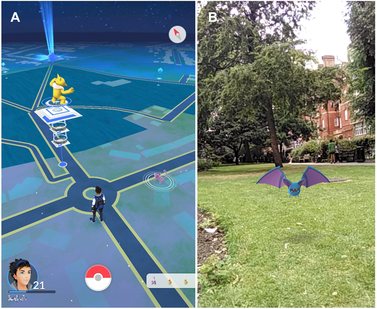
\includegraphics[width=90mm]{./figuras/pokemonGoIntro}
	\caption[Uso de la aplicación Pokémon Go\textcopyright ]{Uso de la aplicación Pokémon Go\textcopyright\ obtenida de \cite{Dorward2017}} \label{fig:pokemonGoIntro}
\end{figure}\\
Hoy en día, la Realidad Aumentada ha adquirido mayor popularidad y expansión debido a las aplicaciones en donde se encuentra. Por ejemplo, en la industria del entretenimiento, específicamente en el área de los videojuegos, existe una aplicación muy popular, conocida como Pokémon GO\textcopyright\ (\cite{Dorward2017}), el cual consiste en la búsqueda y captura de personajes de la saga Pokémon, que se encuentran escondidos en el mundo real, visualizados a través de un smartphone (Figura \ref{fig:pokemonGoIntro}), en donde claramente se puede ver el concepto de Realidad Aumentada debido a que los personajes están superpuestos en nuestro mundo real. Así mismo, encontramos que la AR abarca áreas como la medicina (\cite{Marescaux2004,Ploder1995}), turismo (\cite{Kounavis2012}), manufactura (\cite{Frund2004}), entre muchas otras.\\
Todas estas aplicaciones en donde se encuentra la Realidad Aumentada, son visualizadas a través de dispositivos tales como HMD (Hololens de Microsoft, GoogleGlass de Google), computadoras, tablets o smartphones, y aunque gradualmente se han ido optimizando tanto el hardware como el software de cada uno de ellos, su uso impide al observador tener una conexión más real con su mundo, debido a factores tales como el campo de visión limitado por los mismos dispositivos, latencia en los gráficos que en ocasiones puede provocar mareos, y la necesidad obligatoria de llevar un equipo encima para poder visualizar este tipo de realidad. Debido a lo anterior, existe una variante de ésta tecnología, conocida como Realidad Aumentada Espacial (SAR, Spatial Augmented Reality), que mantiene el mismo concepto de la AR, pero con la diferencia que ésta es mostrada mediante proyectores digitales, es decir, proyecta información u objetos virtuales directamente sobre objetos físicos, por lo tanto, ya no necesitaríamos llevar con nosotros algún dispositivo para visualizarla.\\
En un inicio, SAR, simplemente se utilizaba en la proyección de imágenes o videos que se adaptaban a la forma de fachadas de edificios ofreciendo espectáculos visuales. Pero más adelante se integró la fase de interacción con estos elementos virtuales, lo cual aunque ayudó a involucrarse en varias industrias y expandir su aplicación, aumentó su nivel de complejidad, encontrando varias problemáticas que actualmente siguen en proceso de desarrollo.
%%->Planteamiento del problema
\section{Planteamiento del problema}
La Realidad Aumentada Espacial (SAR), siendo entonces un nuevo paradigma que se deriva de la Realidad Aumentada, es una nueva forma de visualizar elementos virtuales sin la necesidad de verlos a través de dispositivos sujetos a estar en nuestro cuerpo.\\
Estos objetos virtuales proyectados en nuestro entorno, a pesar de jugar en algunos casos con nuestra mente, para dar un efecto 3D, utilizando sombras en lugares específicos y aplicando técnicas para dar profundidad, se puede lograr distinguir de lo real con sólo situarnos en otro lugar en torno a la proyección y verlo desde otra perspectiva. Esto ocasiona por lo tanto que exista aún una gran barrera entre lo que es real y lo que es virtual en términos de SAR.\\
El estudio de proyectar objetos virtuales 3D, que se asemejen tanto a los objetos físicos, pudiendo en algunas ocasiones sustituirlos, es una de las problemáticas actuales sin resolver y que muy pocos han intentado abordar, debido al grado de complejidad que pudiese tener el desarrollo de ésta. Considerando que, para que se pueda implementar esta mejora, se debe tener en cuenta varios aspectos tales como:
\begin{itemize}
\item La deformación de los objetos virtuales al proyectarse directamente sobre los objetos físicos.
\item La detección de una o más personas.
\item El seguimiento de la persona a la cual se le tomará en cuenta la perspectiva, debido a que únicamente se podría proyectar la perspectiva de una sola persona.
\item La calidad de la proyección de los elementos virtuales.
\end{itemize}
Se propone, por lo tanto, a través de un esquema simple inicial y en un futuro, aplicable a cualquier escenario virtual, la proyección de un escenario con elementos 3D, adaptable a la perspectiva de la persona, perfeccionando y cumpliendo aún más con el objetivo del término de Realidad Aumentada Espacial.
%%

%%Justificación
\section{Justificación}
Aunque varios proyectos en donde se aplica SAR, se encuentran dirigidos a la industria de los videojuegos (lo cual, a pesar de lo que muchos opinan ser una pérdida de tiempo, éstos son capaces de desarrollar múltiples habilidades en los usuarios y vivir experiencias únicas), el uso de SAR, se expande a distintas áreas proporcionando enriquecer la experiencia visual, y por lo tanto apoyando el desarrollo y entendimiento de las mismas.\\
Es por ello que proyectar escenarios u objetos virtuales cambiando su ángulo de vista cuando una persona se mueve alrededor de éste, nos brinda la oportunidad de darle más realidad a un objeto virtual y vivir una experiencia mejorada de SAR.\\
En la educación el uso de esta técnica nos permitiría, agilizar el proceso de aprendizaje, debido al impacto que causaría la proyección de objetos virtuales 3D, en temas como figuras o lugares históricos, planetas, el cuerpo humano, entre otros, que dieran la posibilidad de mostrar más información de la proporcionada en una simple imagen, y así motivar su estudio.\\
En la rama de la arquitectura, la visualización de una estructura, ya sea un edificio o casa, proyectada en 3D sin la necesidad de crear una maqueta, ayudaría a ahorrar recursos y vivir la misma experiencia, incluyendo la ventaja de poder modificar su modelado y ver instantáneamente el resultado que obtendrían de manera virtual.\\
Por lo tanto, el desarrollo de mostrar un escenario virtual 3D, según la perspectiva de una persona, sería un paso más hacia la adaptabilidad de un mundo virtual en el mundo real, siendo una potente herramienta de visualización capaz de contribuir en el desarrollo de múltiples áreas.
%%

%%Objetivos
\section{Objetivos}
%General
\subsection{General}
Desarrollar un sistema capaz de determinar el ángulo correspondiente de un entorno virtual basado en la perspectiva de una persona y proyectarlo en nuestro mundo para proporcionar un efecto de realidad.
%
%Específicos
\subsection{Específicos}
\begin{itemize}
\item Determinación de los módulos que intervendrán en el sistema mediante el análisis de los requerimientos.
\item Detección del número de personas en la escena y selección del individuo de interacción, por medio del desarrollo y la implementación de un módulo.
\item Determinar la posición en donde se encuentre la persona y la altura proporcionada por la imagen de profundidad de un sensor RGB - D, por medio del desarrollo e implementación de un módulo.
\item Optimización del sistema por medio de una comparativa de diversas técnicas en cada uno de los módulos del sistema.
\end{itemize}
%
%%
%%Hipótesis
\section{Hipótesis}
Basado en la posición y altura de una persona, obtenidas mediante un sensor RGB – D es posible obtener su perspectiva respecto a un entorno virtual que será proyectado y creará el efecto 3D que tanto se intenta conseguir.
%%
%%%%%%%%%%%%%%%%%%%%%%%%%%%%%%%%%%%%%%%%%%%%%%%%%%%%%%%%%%%%

%%%CAPÍTULO 2 -> MARCO TEÓRICO%%%
\chapter{Marco Teórico}\label{cap.marcoteorico}
Dado que el presente trabajo de tesis, se centrará en el área de la Realidad Aumentada Espacial (SAR), específicamente en la optimización de la percepción de objetos virtuales 3D, será necesario establecer algunas terminologías y trabajos relacionados que sirvan de apoyo para el correcto entendimiento de éste.
%%Antecedentes
\section{Antecedentes}
La presencia de elementos virtuales en nuestras vidas ha tenido gran influencia en el campo de la investigación y gracias al avance que se ha tenido, se ha contribuído en el desarrollo de diferentes técnicas que proporcionen información visual que sirvan de apoyo en múltiples áreas. Una de las primeras tecnologías en las que se pueden visualizar elementos artificiales es la Realidad Virtual (VR), donde se puede definir según \cite{coiffet1995} como ``un mundo que a pesar de no tener ninguna realidad física es capaz de darle al usuario, a través de una estimulación adecuada de su sistema sensorial, la impresión perfecta de estar en interacción con un mundo físico''. Es por ello que VR es mayormente utilizada para la simulación de escenarios que nos ayuden como entrenamiento, nos proporcionen conocimiento de algún tema en específico o simplemente nos trasladen a un lugar en el que podamos ver libremente lo que nos rodea y en muchas ocasiones interactuar. Por ejemplo, en la rama de la medicina, podemos encontrar su aplicación en la formación y experimentación de actividades quirúrgicas; en la robótica, a través de simuladores aéreos, terrestres y submarinos; y muchas mas aplicaciones que son mencionadas en \cite{levis1997}. Sin embargo, en situaciones en donde uno desea adicionar información virtual y así enriquecer elementos de nuestro entorno real, sería realmente difícil y costoso en términos computacionales, recrear un entorno virtual simulando ser totalmente real como el que nuestros ojos ven, por lo que el uso de imágenes obtenidas mediante sensores y la superposición de elementos virtuales es la técnica utilizada por parte de una tecnología que hoy en día se le conoce como Realidad Aumentada, y que igual que VR, sirve de apoyo en múltiples áreas.
\begin{figure}[th]
	\centering
	\subfigure[Imagen original ]{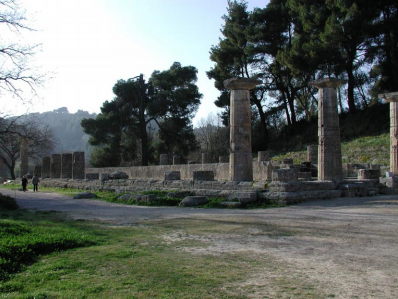
\includegraphics[width=67.5mm]{./figuras/arqueologiaA}}
	\subfigure[Imagen con realidad aumentada ]{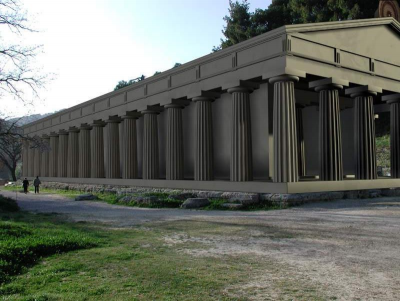
\includegraphics[width=67.5mm]{./figuras/arqueologiaB}}
	\caption[Realidad Aumentada en la arqueología]{Realidad Aumentada en la arqueología: Sistema Archeoguide desarrollado por \cite{vlahakis2002}, el cual reconstruye las ruinas en lugares históricos} \label{fig:arqueologia}
\end{figure}
\subsection{Realidad Aumentada}
La Realidad Aumentada (AR), ha sido definida por varios autores desde distintos puntos de vista \citep{milgram1994,azuma1997}. Algunos, la describen como una variante de la Realidad Virtual (VR); otros la consideran como un concepto general, en donde VR se encuentra dentro de ésta tecnología. Ramesh Raskar, en su libro \citep{Bimber2005} menciona que AR, a diferencia de VR (que crea un entorno virtual desde cero), incorpora en nuestro entorno elementos sintéticos; es decir, superpone objetos o información virtual en una secuencia de imágenes capturadas en tiempo real de nuestro propio entorno, creando la ilusión de que ambos mundos (virtual y real) se fusionan en uno, es decir, creando una realidad mixta (MR). De éste modo, no se pierde la conexión con nuestro mundo en ningún momento, existiendo aplicaciones que contribuyen en el desarrollo y optimización de áreas, como por ejemplo en la arqueología, en donde es utilizada para la reconstrucción de lugares históricos (véase Figura \ref{fig:arqueologia}) o viajar en el tiempo utilizando la información del entorno actual y simular lo que pasó hace miles de años \citep{vlahakis2002}. En cuanto a la rama de la medicina, AR es aplicada en múltiples actividades tales como simuladores de examen de mama, manipulación virtual de la anatomía humana, entre otras aplicaciones que se mencionan en \cite{bichlmeier2007}, las cuales pueden servir como entrenamiento o como herramienta de aprendizaje.
\begin{figure}[th]
	\centering
	\subfigure[Simulador clínico de examen de mama, extraído de \cite{kotranza2009} ]{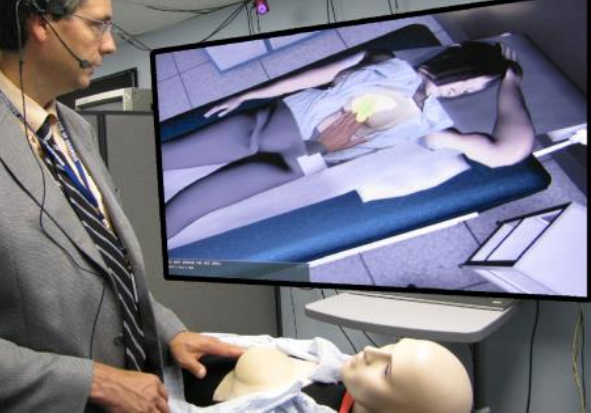
\includegraphics[width=60mm]{./figuras/medicinaAR1}}
	\subfigure[Simulador de operación, explicado en \cite{bichlmeier2007} ]{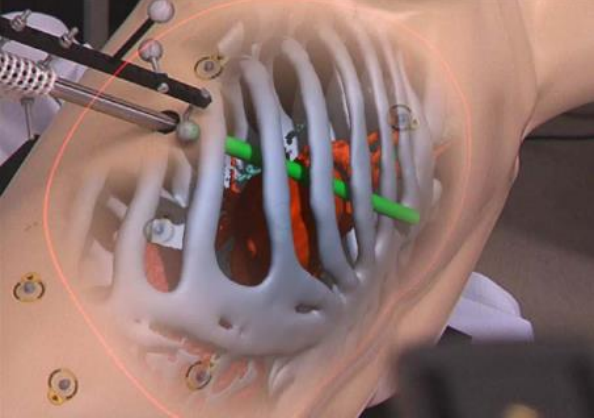
\includegraphics[width=60mm]{./figuras/medicinaAR2}}
	\caption[Realidad Aumentada aplicada a la medicina]{Realidad Aumentada aplicada en la medicina} \label{fig:medicinaAR}
\end{figure}\\
\subsubsection{Técnicas de visualización}
Según Azuma \cite{azuma2001}, existen 3 principales formas en las que podemos visualizar la AR. Tales son a través de: dipositivos utilizados en la cabeza (head-worn displays, HWD), dispositivos de mano (handheld displays) o dispositivos de proyección (projective displays). La manera tradicional de percibir esta realidad es a través de las dos primeras clasificaciones mencionadas anteriormente (en inglés See-though Augmented Reality, STAR \cite{Sol2016}), mientras que la última es mayormente conocida como Spatial Augmented Reality (SAR).\\
\begin{figure}[thbp]
	\centering
	\subfigure[Optical see-through ]{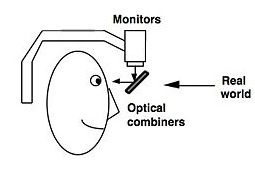
\includegraphics[width=67.5mm]{./figuras/optical}}
	\subfigure[Video see-through ]{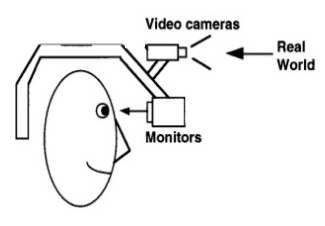
\includegraphics[width=67.5mm]{./figuras/video}}
	\caption[Funcionamiento de los HMD's]{En (a) la superposición AR es proporcionada a través de una pantalla transparente, mientras que (b) las imágenes son capturadas por la cámara de video y usadas como fondo para la superposición AR. Ambas imágenes han sido obtenidas y modificadas de \cite{azuma1997} } \label{fig:opticalvideo}
\end{figure}
\paragraph{See-though Augmented Reality.}
En el caso de los HWD's, en sus inicios se denominaban de ésta manera, pero hoy en día no se utiliza mucho éste término, por lo que otra forma de llamarlo sería como dispositivos montados en la cabeza head mounted displays (HMD), que abarca desde los cascos (utilizados principalmente en el ámbito militar), hasta los lentes que pueden variar su tamaño y sus dimensiones dependiendo de la empresa. Éstos son clasificados por dos tipos de técnicas de visualización: optical see-through y video see-through (Figura \ref{fig:opticalvideo}), en donde su principal diferencia radica en la forma en la que se captura la imagen del mundo real. Comercialmente hablando y los mas populares que podemos encontrar hoy en día, tenemos los Hololens de Microsoft\textcopyright\ y los Google glass\textcopyright\ (Figura \ref{fig:lentesAR}).
\begin{figure}[thbp]
	\centering
	\subfigure[Hololens de Microsoft\textcopyright]{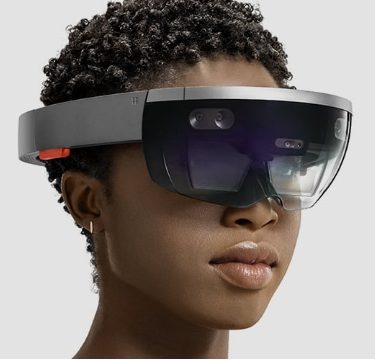
\includegraphics[width=50mm,height=45mm]{./figuras/hololens}}
	\subfigure[Google GLASS\textcopyright ]{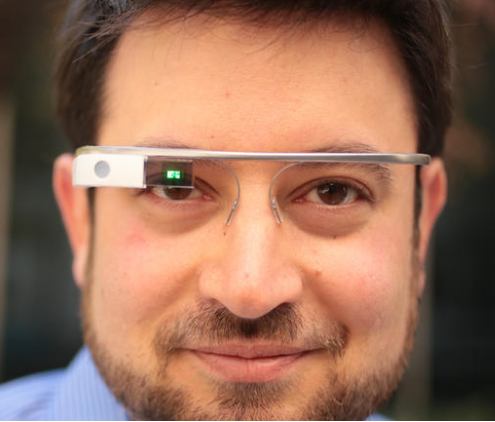
\includegraphics[width=50mm,height=45mm]{./figuras/googleglass}}
	\caption[Lentes de Realidad Aumentada]{Lentes de Realidad Aumentada: (a) Utiliza una técnica avanzada de optical projection \hyperlink{e07}{[E07]}; (b) Utiliza una proyección micro-óptica \hyperlink{e08}{[E08]}} \label{fig:lentesAR}
\end{figure}\\
En cuanto a los handhelds displays, traducido al español como dispositivos de mano, encontramos una amplia diversidad de dispositivos de varias marcas por parte de smartphones y tablets, que debido al bajo costo (en comparación con los HMD's) y al uso común de ellos en nuestras vidas, la AR se ha expandido y dado a conocer por medio del desarrollo de aplicaciones, que así como se ha utilizado como medio de entretenimiento (Pokémon Go\textcopyright, Snapchat\textcopyright, mostradas en la figura \ref{fig:ARejemplos}(a,b)), también ha servido de apoyo en el campo de la enseñanza, siendo capaz de proporcionar información virtual que ayude al entendimiento o aprendizaje en distintas áreas (figura \ref{fig:ARejemplos}(c,d)). Sin embargo, aunque cada vez surgen mas aplicaciones entorno a estos artefactos, el uso de ellos impide al observador tener una conexión mas real con su mundo, debido principalmente al campo de visión limitado por los mismos.\\
\begin{figure}[t]
	\centering
	\subfigure[Pokemon Go\textcopyright  ]{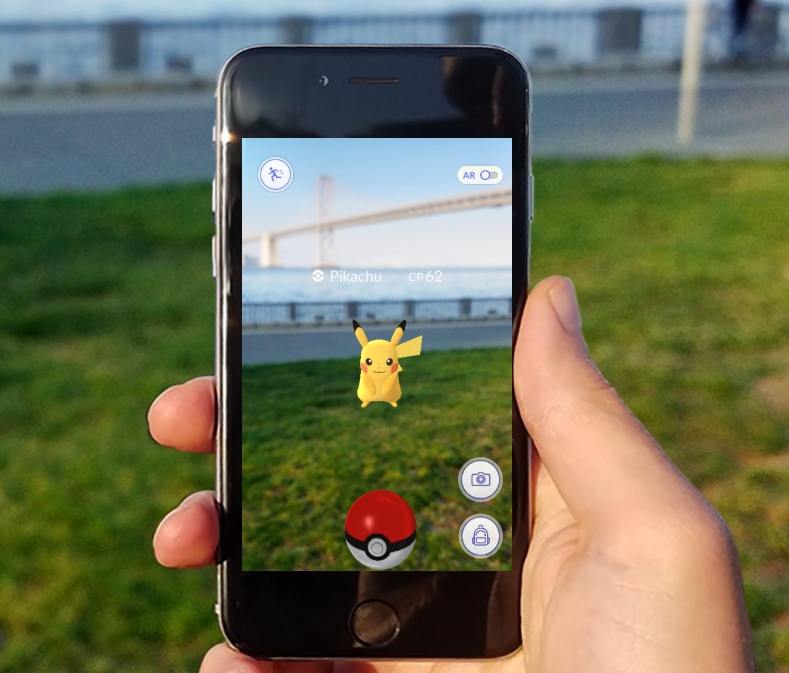
\includegraphics[width=30mm,height=30mm]{./figuras/pokemon}}
	\subfigure[Snapchat\textcopyright ]{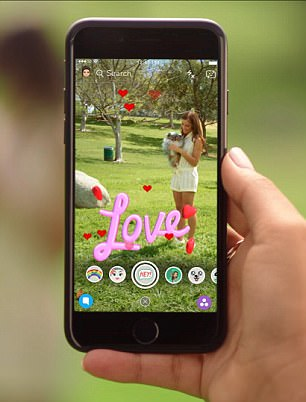
\includegraphics[width=30mm,height=30mm]{./figuras/snapchat}}
	\subfigure[LearnAR\textcopyright ]{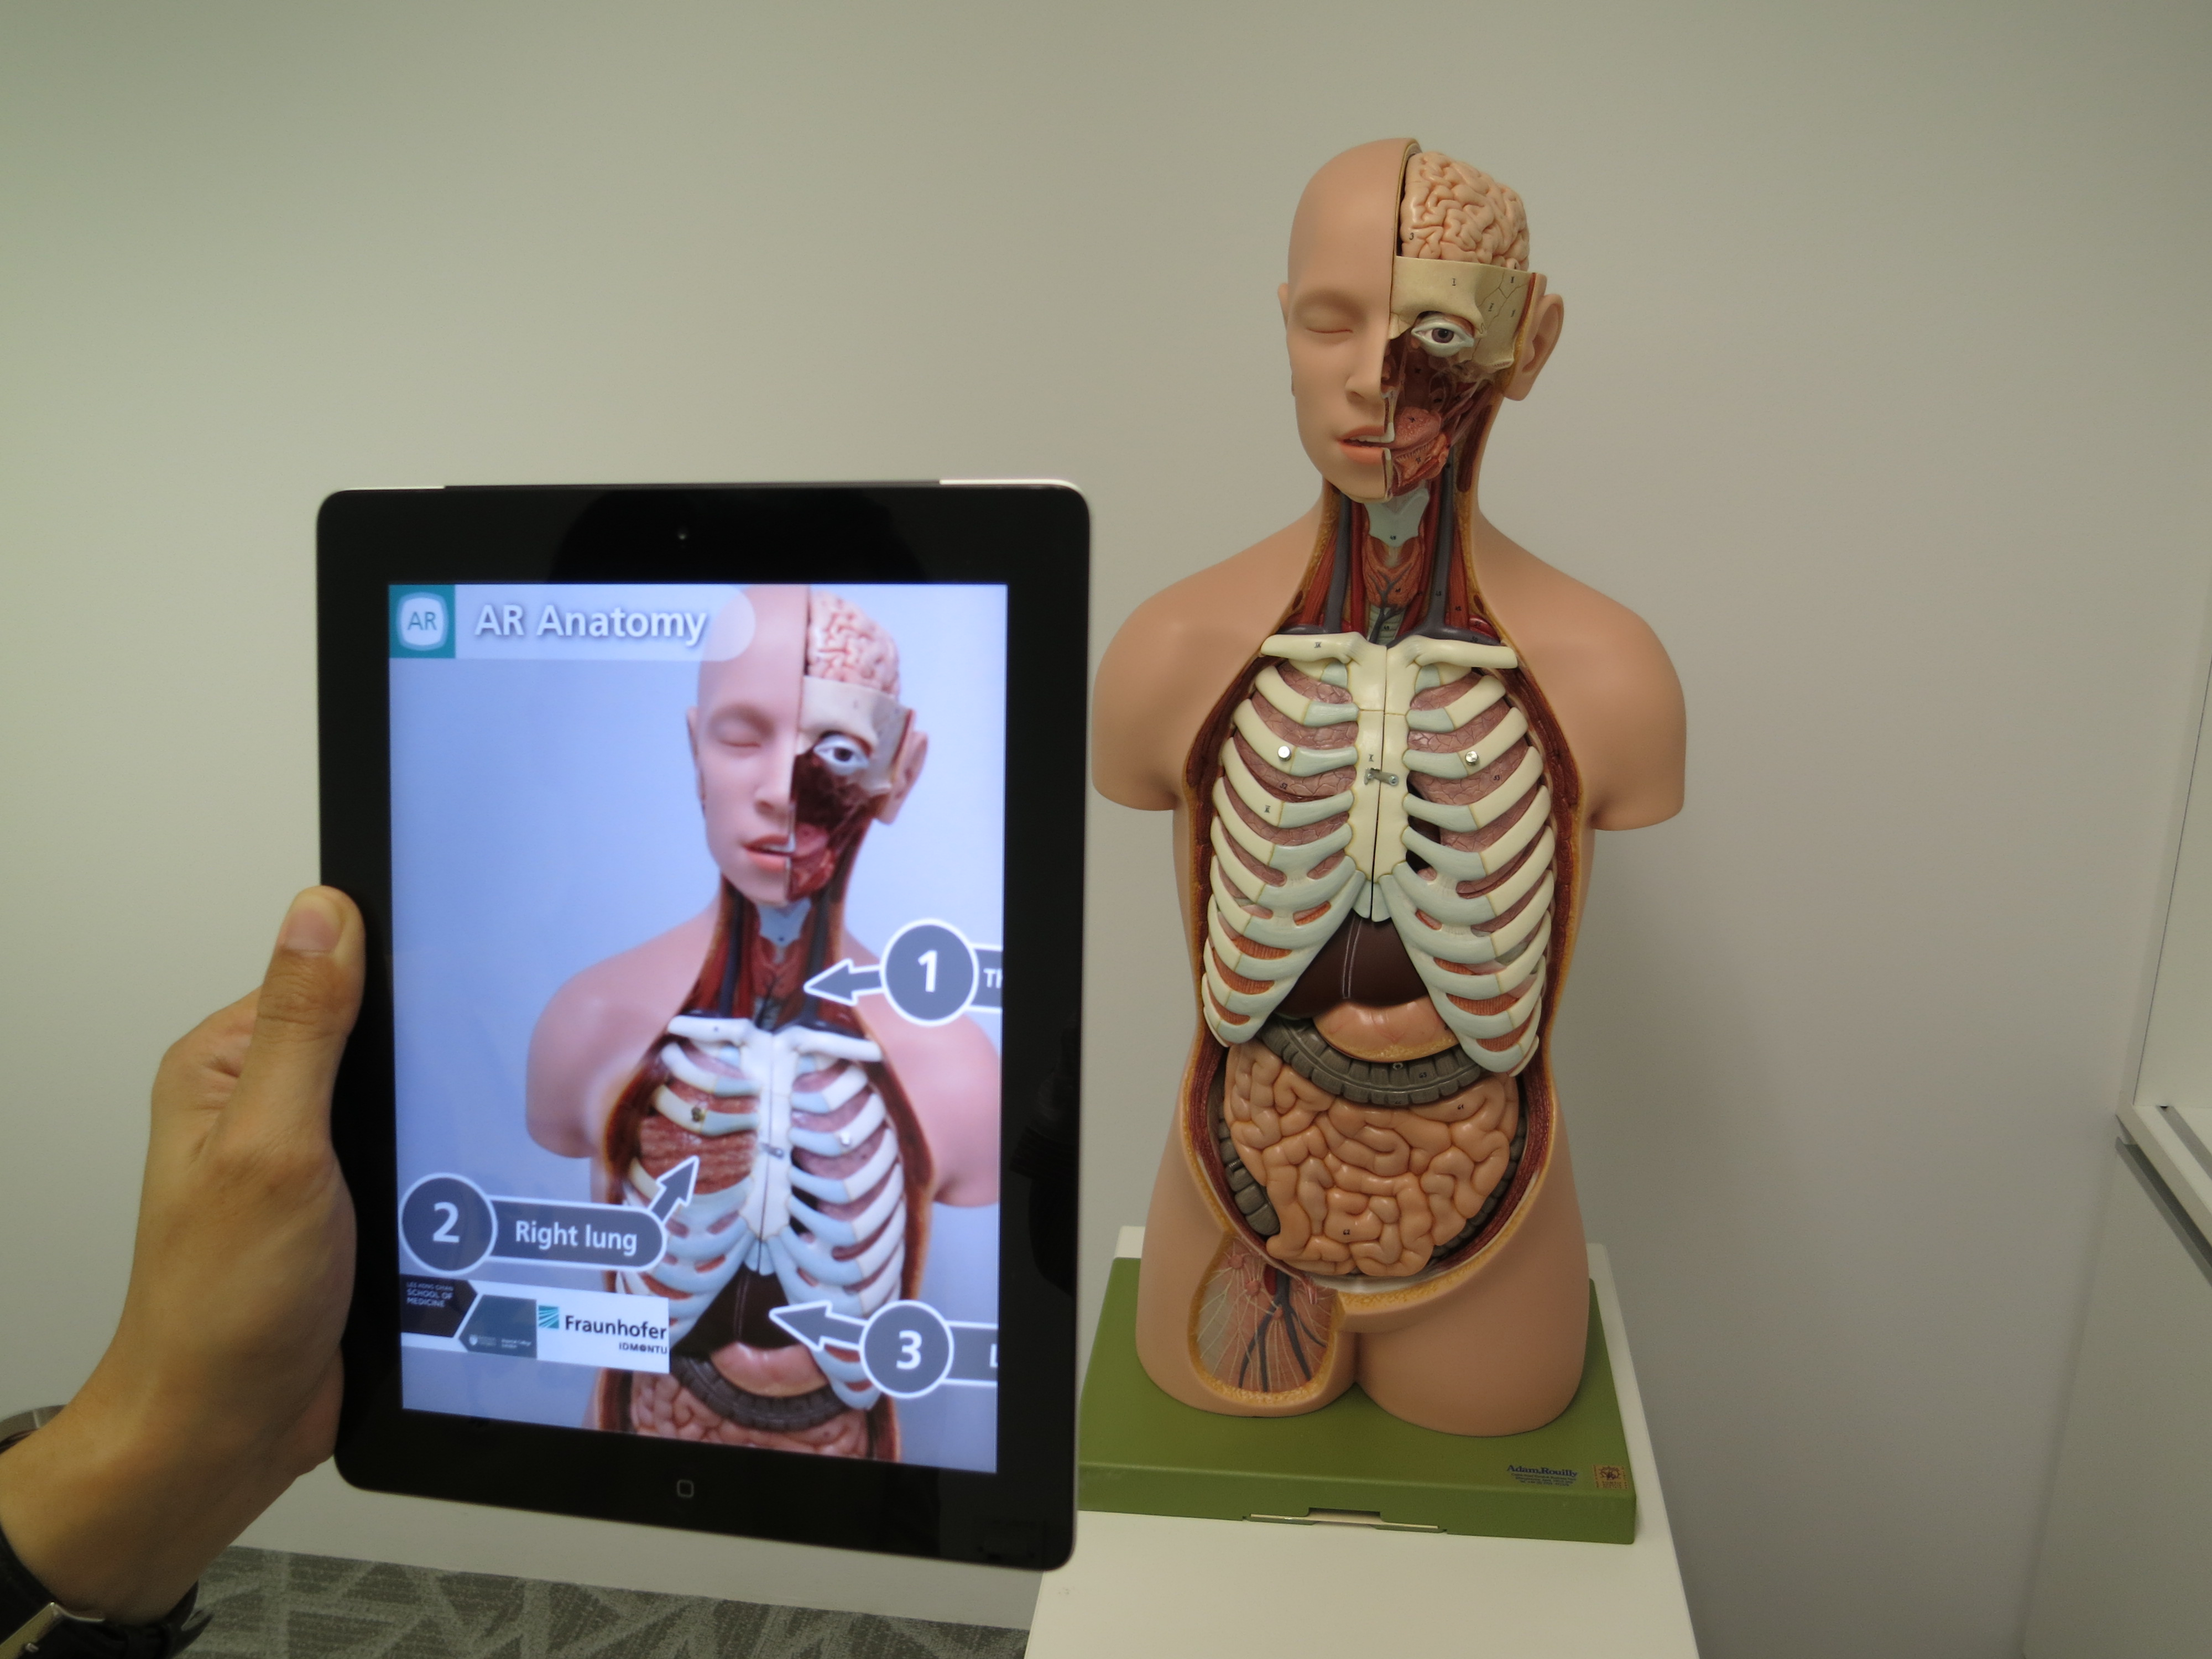
\includegraphics[width=30mm,height=30mm]{./figuras/learnAR}}
	\subfigure[Google Translater \textcopyright ]{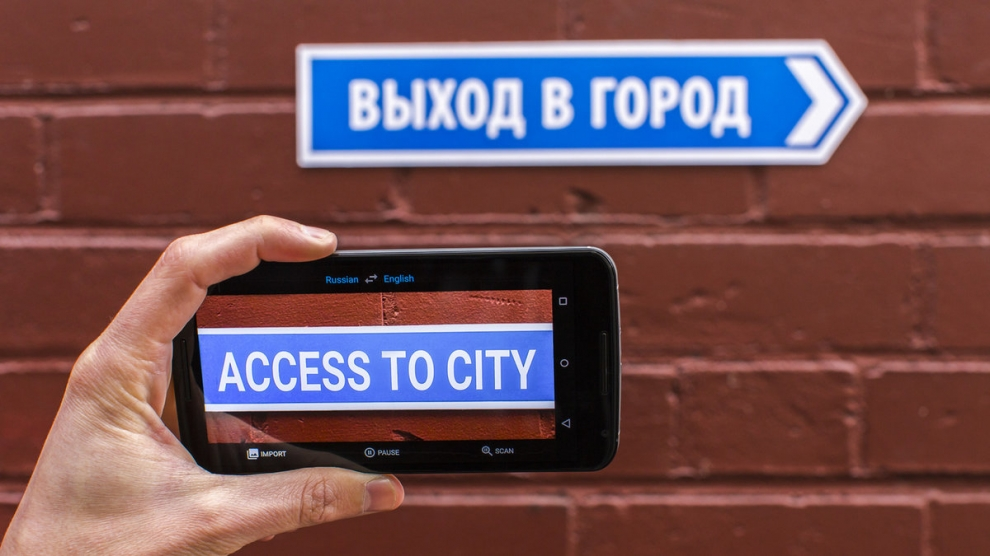
\includegraphics[width=30mm,height=30mm]{./figuras/googleTranslater}}
	\caption[Ejemplos de AR en smartphones y tablets]{Los ejemplos (a)\hyperlink{e02}{[E02]} y (b)\hyperlink{e03}{[E03]} están enfocados al entretenimiento; (c)\hyperlink{e04}{[E04]} y (d)\hyperlink{e05}{[E05]} están enfocados a la educación} \label{fig:ARejemplos}
\end{figure}

\section{Estado del arte}
La Realidad Aumentada Espacial (SAR), es una variante de la AR, que muestra mediante proyectores digitales, información u objectos virtuales directamente sobre objetos físicos, lo cual una de las ventajas que trae consigo con respecto a STAR, es el hecho de no tener que llevar un equipo encima para poder visualizar este tipo de realidad, además de poder involucrar la libertad de poder interactuar directamente (sentido del tacto) de tal modo que nos ayude a estar mas en contacto con los objetos virtuales.\\
Raskar fue uno de los primeros en dar a conocer este nuevo paradigma a través de varios prototipos \citep{Raskar1998a,Raskar1998b,Raskar2001}, los cuales se basan principalmente en resolver problemas en cuanto a la distorsión de la imagen en la irregularidad de la superficie. Mas adelante, se implementó la fase de interacción entre el usuario y los elementos virtuales, lo cual atrajo la atención de grandes compañías tales como Microsoft\textregistered, Sony\textregistered, Disney\textregistered, pero a la vez, surgieron problemas mas complejos que aún siguen en proceso de investigación y desarrollo.\\ 
Dependiendo del uso o la aplicación en donde se encuentre ésta tecnología, se le atribuyen otros nombres que ayuden a entender de forma mas clara su propósito en donde se esté implementando. Ésto debido a que cuando hablamos de ``Espacial'' (palabra que forma parte del término Realidad Aumentada Espacial), no solo nos estamos refiriendo a la percepción de información adicional a través del sentido visual, sino que también podemos involucrar el tacto y el sentido auditivo.\\ 
\subsection{Projection mapping}
Comercialmente SAR, también es conocida como ``projection mapping'' o ``video mapping'', refiriéndose a la proyección de información virtual en objetos reales, con el objetivo de enriquecerlos visualmente, mostrando una nueva forma de percibir el objeto. De igual manera se pueden proyectar imágenes o elementos virtuales en superficies tales como paredes de edificios para publicidad, como medio artístico en escenarios o incluso en el rostro o cuerpo de las personas (Figura \ref{fig:projectionmapping}). Para ver toda la información respecto a ésta tecnología, el sitio oficial de Projection Mapping \hyperlink{e01}{[E01]} exhibe muchos proyectos interesantes.
\begin{figure}[h]
	\centering
	\subfigure[OMOTE]{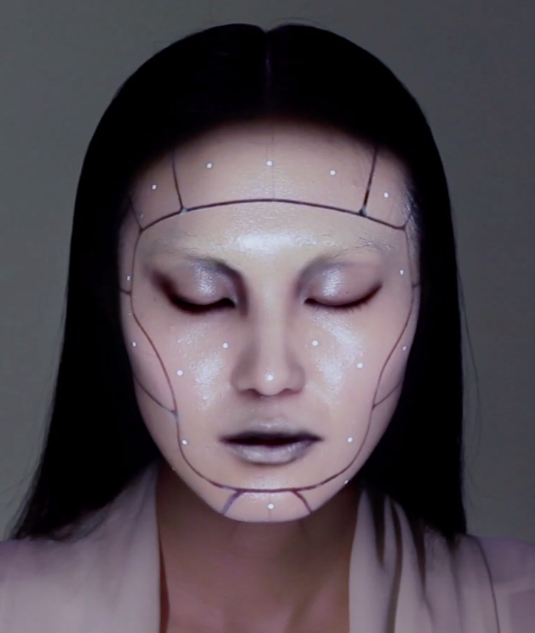
\includegraphics[width=35mm,height=40mm]{./figuras/projectionmapping1}}
	\subfigure[Bonython Hall]{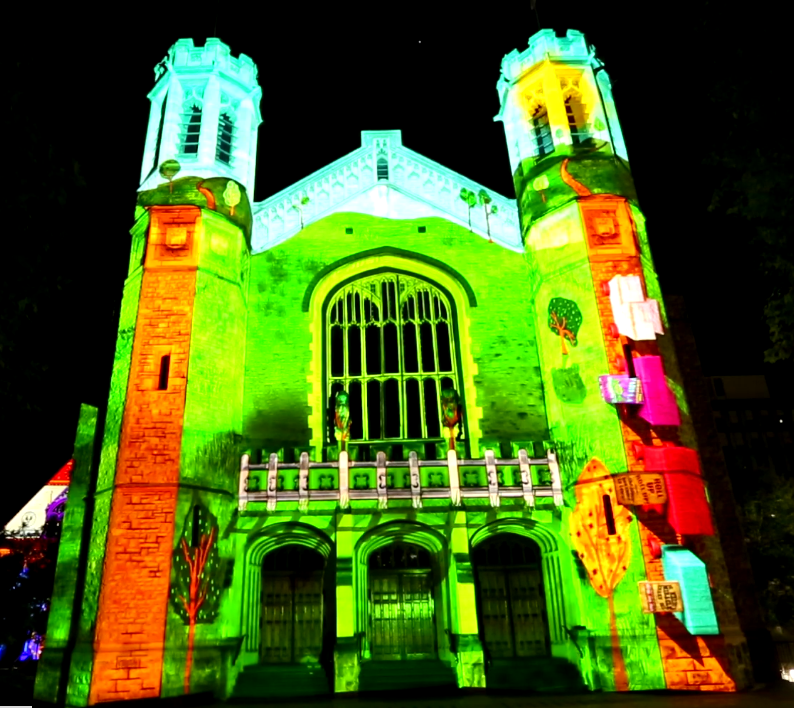
\includegraphics[width=40mm,height=40mm]{./figuras/projectionmapping2}}
	\subfigure[Proyecto de KnownSense]{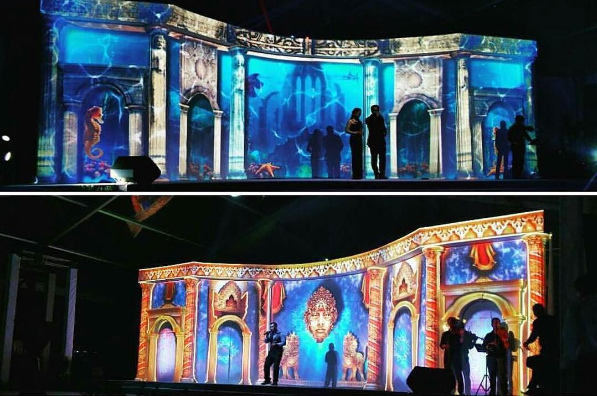
\includegraphics[width=55mm,height=40mm]{./figuras/projectionmapping3}}
	\caption[Ejemplos de Projection Mapping]{Ejemplos de Projection Mapping: (a) desarrollado por el artista Nobumichi Asai (Japón); (b) proyecto expuesto en el Festival Adelaide (Australia); (c) desarrollado por KnownSense Studios; (todas las imágenes fueron obtenidas del sitio oficial \hyperlink{e01}{[E01]})} \label{fig:projectionmapping}
\end{figure}\\
Su nivel de complejidad, por lo tanto, varía dependiendo de la superficie en donde pueda ser proyectada la información y en algunos casos, para facilitar y obtener una proyección adaptativa en tiempo real, se suelen utilizar guías o marcadores (Figura \ref{fig:projectionmapping}(a)) para realizar cálculos mas exactos de los límites en donde se proyectaría la imagen. Inicialmente, las propuestas a los problemas en la proyección eran tratados de forma independiente, es decir, los proyectos presentados únicamente atacaban un problema a la vez. Por ejemplo, Luminous Room propuesto por \cite{Under1997} proyectaba la información en una superficie plana, donde únicamente se ajustaba la deformación que ocasionaba la proyección dependiendo de donde se encontrara el proyector. Sin embargo, años antes, se propuso un análisis de la estructura del escenario propuesto por \cite{Dorsey1991} (en éste caso pantallas curvas) para proyectar información, en donde generaban las imágenes pre-distorsionadas para que luego se pudiesen visualizar de la forma correcta. En cambio, cuando la superficie en donde se proyecta la información posee objetos y por lo tanto se muestra de forma irregular, varias propuestas tratadas de manera subsecuente sirvieron para obtener una correcta proyección; ésto es a través de un análisis previo de su forma para así capturar la información 3D de los objetos físicos, pre-distorsionar la imagen conforme a la irregularidad del escenario, tomar en cuenta la posición en donde se encuentra la persona y seguido a esto, la proyección correcta de los elementos virtuales \citep{Raskar1998b,Raskar2001,Starner2003,Wilson2007}.\\
IllumiRoom \cite{jones2013}, es un claro ejemplo en donde la información virtual se adapta en nuestro entorno, tomando en cuenta la geometría y apariencia de éste, con el objetivo de aumentar la zona que rodea una pantalla de televisión y mostrar un escenario extendido de éste (Figura \ref{fig:illumiRoom}.
\begin{figure}[thb]
	\centering
	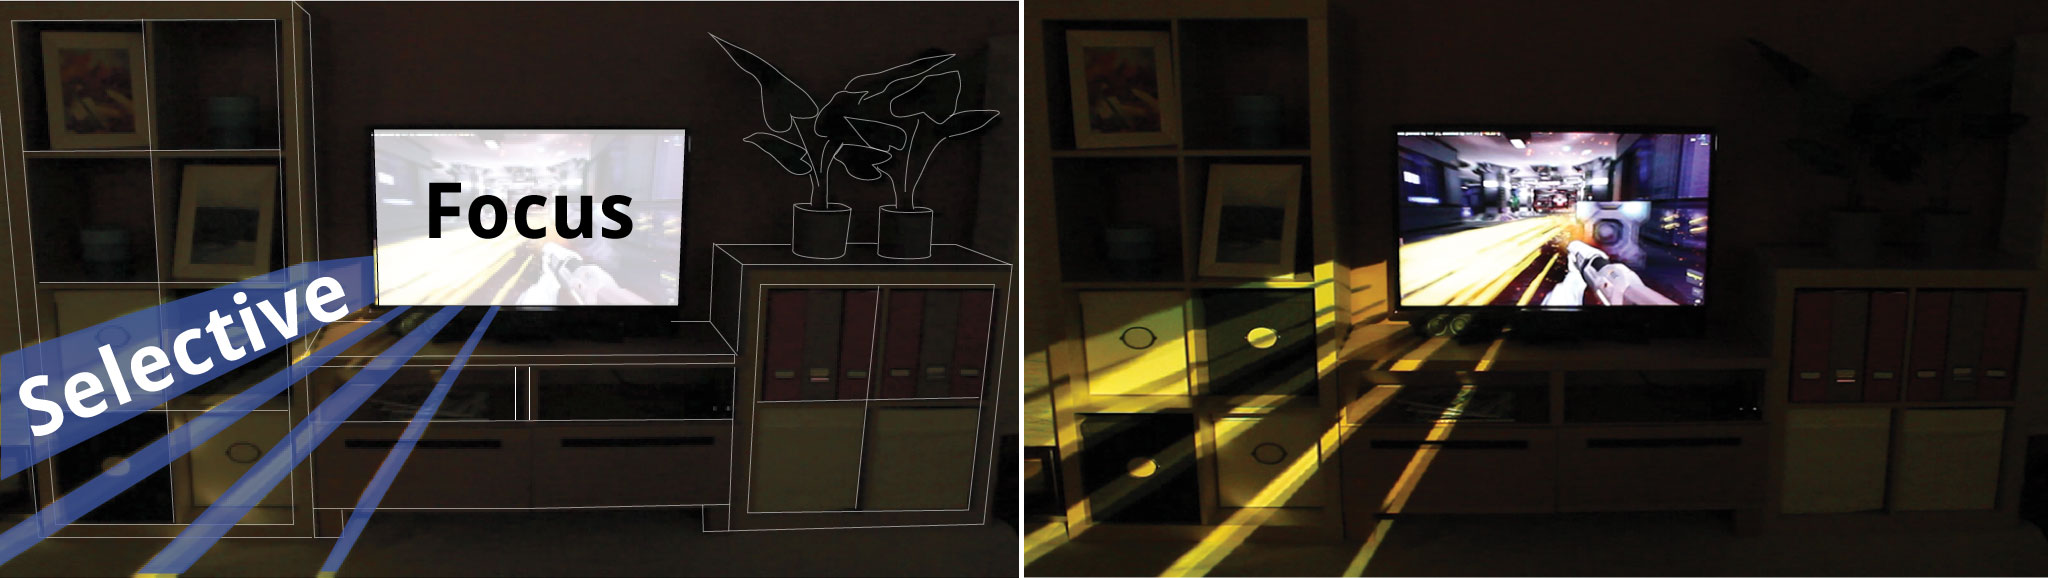
\includegraphics[width=140mm]{./figuras/illumiRoom}
	\caption[Proyecto IllumiRoom por Microsoft\textregistered]{IllumiRoom: proyecto desarrollado por Microsoft\textregistered, ejemplo de funcionamiento \hyperlink{e09}{[E09]} } \label{fig:illumiRoom}
\end{figure}
\subsection{Interacción en SAR}
En sus primeros años de desarrollo, no se contaba con una fase de interacción entre el usuario y los elementos virtuales, debido a que su propósito en ese momento, era mostrar información adicional, aumentando la experiencia visual. Fue entonces, que gracias a grandes compañías tales como Microsoft Research\textregistered, desarrollaron proyectos y propusieron nuevas técnicas que incluían la interacción a través de las manos, voz o algún dispositivo de apoyo, lo cual propició la expansión de SAR en distintas áreas, principalmente en el aprendizaje y entretenimiento. Debido a que la información virtual mostrada depende de la superficie en donde será proyectada, existen proyectos en los que se pueden visualizar los elementos virtuales en mesas o superficies planas para poder interactuar con ellos de un manera mas fácil y controlada. Por otra parte, existen proyectos enfocados a las superficies irregulares, los cuales requerirán de una serie de análisis y cálculos previos que a diferencia de los de sobremesa, éstos resultarán ser más complejos de desarrollar. Generalmente los prototipos desarrollados por los investigadores que, a través de ellos proponen técnicas para solucionar los problemas en éstos escenarios, no toman en cuenta la perspectiva de la persona con respecto a los elementos virtuales que se encuentren presentes en nuestro mundo, por lo cual la libertad de poder ver e interactuar con ellos resulta limitada si lo que se necesita es visualizarlos como objetos reales.\\
\subsubsection{Proyecciones de Sobremesa}
Mucho del desarrollo y avance de SAR, se inició a través de proyectos que mostraban la información en sobremesa (tabletops) y éstas eran visualizadas a través de proyectores que generalmente estaban ubicados en el techo, proyectando la información encima de la mesa (front-projected displays) o debajo de ésta (técnica conocida como retroproyección).
\begin{figure}[th]
	\centering
	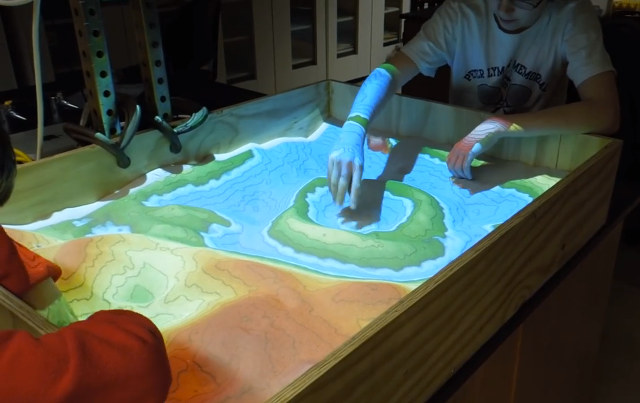
\includegraphics[width=90mm,height=60mm]{./figuras/sandbox}
	\caption[Proyecto de sobremesa: SandBox]{Proyecto de sobremesa: SandBox, desarrollado por la Universidad de California en Davis que simula un modelo topográfico \hyperlink{e10}{[E10]} } \label{fig:sandbox}
\end{figure}\\
Augmented Reality SandBox \cite{kreylos2016}, es un proyecto, basado en front-projection, que actualmente se encuentra en algunos museos, desarrollado por investigadores de la Universidad de California en Davis, en el cual proponen una interactiva forma de aprender topografía, ésto, utilizando arena en una caja especial, creando un modelo topográfico en relación a la forma en la que se encuentre la arena, es decir, dependiendo de la altura del relieve detectado por un sensor de profundidad, es proyectada la información real de cómo se comportaría el terreno (ver Figura \ref{fig:sandbox}).\\
La proyección frontal, en la mayoría de los proyectos ocasiona que las manos u otras partes del cuerpo de las personas, obstruyan la proyección (en el mismo SandBox, se pudo notar ésto), ocasionando poca realidad de inmersión de elementos virtuales en nuestro entorno \citep[ejemplos de proyección frontal]{dietz2001,wilson2005,kreylos2016}. Como una propuesta de solución a éste problema, MirageTable (\cite{benko2012}) proyecto desarrollado por Microsoft Research\textregistered, proponen una técnica, que es capaz de manipular los elementos virtuales como si fuesen objetos reales, adoptando las características físicas que pudiesen tener, tomando en cuenta la interacción y superposición de estos en las manos, sin la distorsión que causaría ésta (Figura \ref{fig:mirageTable}).
\begin{figure}[th]
	\centering
	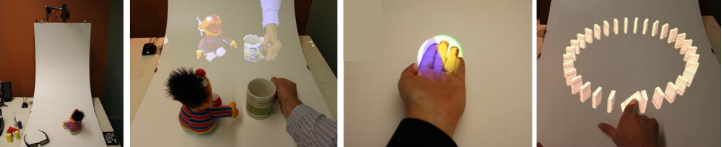
\includegraphics[width=140mm]{./figuras/mirageTable}
	\caption[Proyecto de sobremesa: MirageTable]{Proyecto de sobremesa: MirageTable, desarrollado por Microsoft Research\textregistered, sistema que escanea cualquier objeto en la superficie de la mesa y superpone los objetos proyectados en las manos con interacciones físicas reales \citep{benko2012}} \label{fig:mirageTable}
\end{figure}\\
En lo que respecta a la técnica de la retroproyección, según el Diccionario de fotografía y diseño \hyperlink{e11}{[E11]}, se define como ``la proyección de una imagen por la parte trasera de una pantalla traslúcida que servirá de fondo a un motivo situado por su parte delantera'', de ésta manera la obstrucción de nuestras manos en la proyección ya no sería un problema. Tomando el ejemplo anterior, trabajo previo a MirageTable, fue propuesto una robusta técnica de manipulación de objetos virtuales para este tipo de proyección, simulando la manera en la que nosotros utilizamos los objetos físicos \citep{hilliges2009}. También, encontramos que el uso de la retroproyección, ha servido para mostrar información virtual con múltiples usuarios, optimizando las técnicas de seguimiento de manos y reconocimiento de gestos, para un correcto uso multi-touch, apoyando el trabajo colaborativo \citep[ejemplos de retroproyección]{geller2006,dohse2008}.
\subsubsection{Proyecciones en superficies irregulares}
\begin{figure}[th]
	\centering
	\subfigure[Estructura del escenario de RoomAlive]{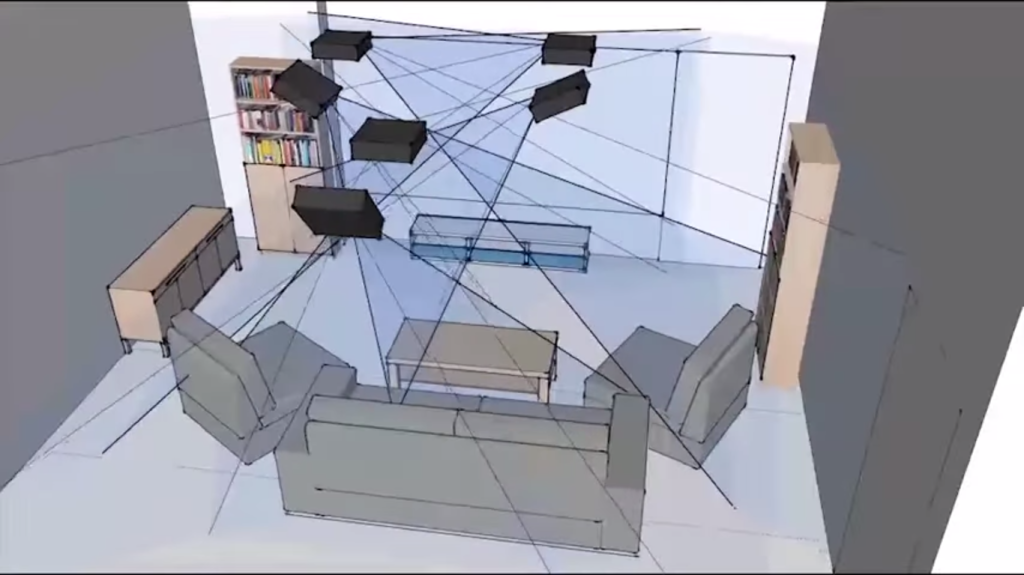
\includegraphics[width=67.5mm]{./figuras/roomalive1}}
	\subfigure[Juego experimental de RoomAlive]{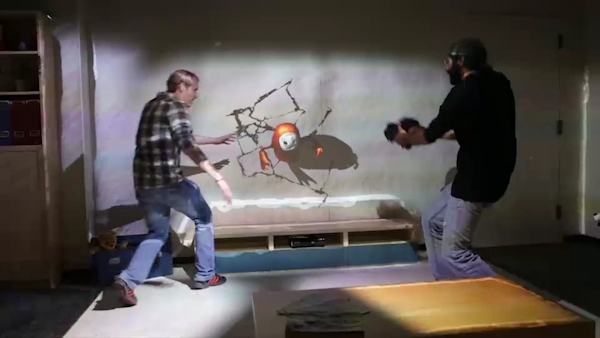
\includegraphics[width=67.5mm]{./figuras/roomalive2}}
	\caption[Proyecto RoomAlive por Microsoft\textregistered]{Proyecto RoomAlive por Microsoft\textregistered; (a) escenario conformado por 6 unidades procam (una unidad procam posee un proyector (pro) y un sensor Kinect\textcopyright(cam)); (b) juego experimental que identifica superficies planas, proyecta objetos en ella y se puede interactuar con estos elementos) \hyperlink{e12}{[E12]}} \label{fig:roomalive}
\end{figure}
Debido a la necesidad de llevar la tecnología SAR a nuestros hogares, principalmente como medio de entretenimiento, se han propuesto y desarrollado varias técnicas, en donde una de las principales cuestiones en las que se ha enfocado el estudio, es en la detección y modelado de la geometría de los objetos físicos, e incluso en la detección y ubicación de elementos en nuestro entorno, para involucrar a los elementos virtuales en nuestro medio, con el objetivo de que se puedan desenvolver de una forma mas real.\\
RoomAlive, es un complejo proyecto propuesto por Microsoft Research\textregistered, que es capaz de transformar cualquier habitación en un área de entretenimiento de realidad aumentada espacial \cite{jones2014}. Poseen un sistema de seguimiento de personas que es utilizado para que el escenario cambie dinámicamente alrededor de ellos. El sistema, se basa principalmente en identificar superficies planas como paredes y piso, esto a través de una combinación de mapas de profundidades de 6 sensores RGB-D distribuidos por toda la habitación, de manera que se puedan clasificar las superficies, y así brindar la oportunidad de crear situaciones y escenarios virtuales mas reales (Figura \ref{fig:perspectiva}).
\subsubsection{Proyecciones en torno a la perspectiva}
A pesar de que se ha logrado un buen avance en la proyección de elementos virtuales en nuestro entorno, de tal forma que no se distorsionen al ser mostrados en tiempo real, no se ha abarcado mucho en el estudio que toma en cuenta al objeto virtual 3D, mostrando sus respectivos ángulos o lados en torno a la perspectiva de una persona.
\begin{figure}[thb]
	\centering
	\subfigure[Estructura del escenario de proyecto VAM]{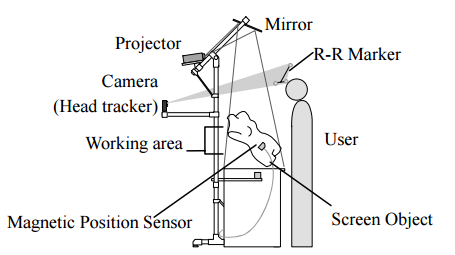
\includegraphics[width=100mm]{./figuras/vam1}}
	\subfigure[Ejemplo de proyección de modelo anatómico]{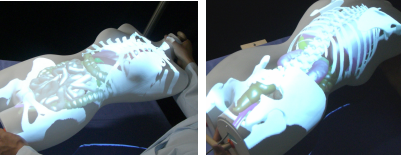
\includegraphics[width=100mm]{./figuras/vam2}}
	\caption[Proyecto Virtual Anatomical Model]{Proyecto Virtual Anatomical Model, que muestra la anatomía del ser humano tomando la perspectiva del observador; en (b) se puede observar que muestra la información dependiendo del lado (frontal o trasero) \cite{kondo2008}} \label{fig:vam}
\end{figure}\\
Uno de los primeros proyectos, en el cual que se empezó a tomar en cuenta éste estudio, lo podemos encontrar por parte de la Universidad de Gifu (Japón), con un prototipo llamado Virtual Anatomical Model(VAM) en su artículo \cite{kondo2008}, el cual ésta enfocado en el área de la medicina y se basa principalmente en combinar un objeto físico con forma humana (maniquí), el cual se encuentra encima de una mesa y superponer la información virtual directamente en el objeto mostrando los órganos internos del cuerpo humano para facilitar el aprendizaje de éstos. Proponen a través de marcadores en un gorra del observador realizar un seguimiento de la cabeza para así mostrar correctamente la perspectiva dependiendo de la posición en donde se encuentre, y de ésta forma exista una mejor interacción con lo observado. En la figura \ref{fig:vam} se muestra cómo fue construido el sistema en general y cómo se muestra la información.
\begin{figure}[htb]
	\centering
	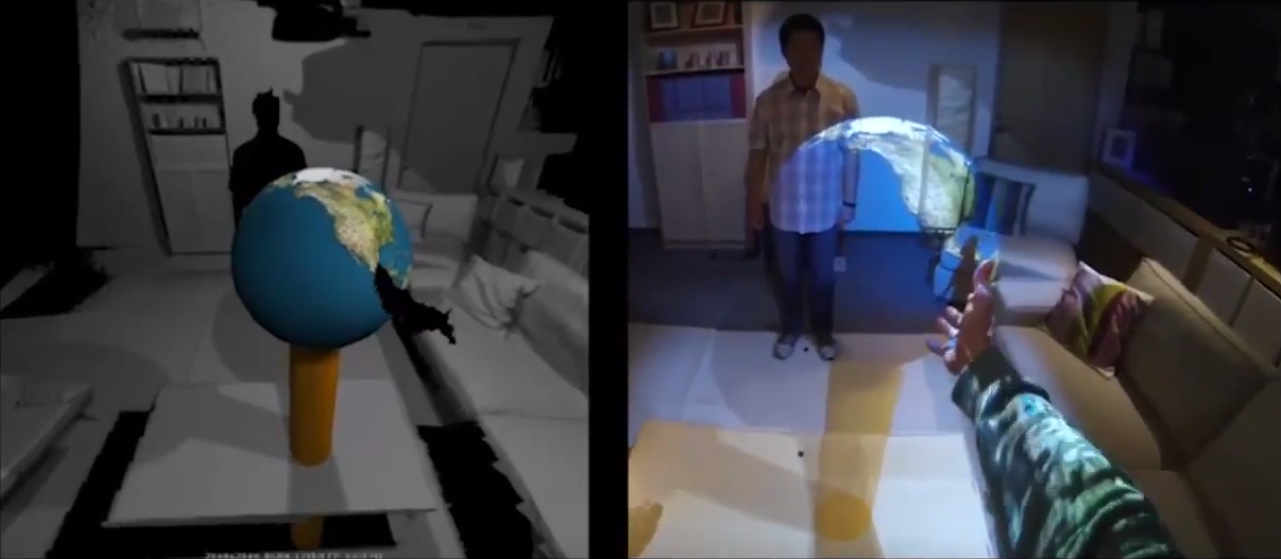
\includegraphics[width=130mm]{./figuras/dyadic1}
	\caption[Proyecto Mano-a-mano por Microsoft\textregistered]{Proyecto Mano-a-mano por Microsoft\textregistered; la imagen de la izquierda es la simulación virtual del escenario, mientras que la derecha es la proyección de éste en un entorno real} \label{fig:perspectiva}
\end{figure}\\
Por parte de Microsoft\textregistered, contamos con un proyecto llamado Mano-a-mano \citep{benko2014}, el cual involucra las técnicas anteriormente mencionadas en RoomAlive y adicionalmente se realiza una adaptación del elemento virtual con respecto a la posición de la persona. En ésta propuesta, es tomada la perspectiva de dos personas que se encuentran una frente a la otra, lo cual involucra la interacción multi-usuario y la posibilidad de visualizar los objetos virtuales tal como si fuesen reales. Sin embargo, el ángulo en el que se pueden desplazar es limitado (menos de 90 grados) debido a la posición de los proyectores (parte de la imagen es proyectada directamente sobre la persona contraria), por lo tanto la interacción y visualización de los objetos virtuales 3D sigue siendo tema de estudio (Figura \ref{fig:perspectiva}).%%
%%%%%%%%%%%%%%%%%%%%%%%%%%%%%%%%%%%%%%%%%%%%%%%%%%%%

%%%CAPÍTULO 3 -> DISEÑO%%%
\chapter{Dise\~no}\label{cap.diseno}
El correcto diseño de un sistema así como el análisis de los elementos que lo conformarán, es de suma importancia, para su futura escalabilidad y optimización. Éste trabajo de tesis fue realizado a través de módulos los cuales permitan ser mejorados de forma independiente evitando a todo costo que la modificación de alguno de ellos afecte el funcionamiento de todo el sistema en general.\\
%%
\section{Análisis de Requerimientos}
Antes de iniciar el desarrollo de cualquier sistema, se debe realizar un análisis de los elementos que estarán involucrados en éste para su correcto funcionamiento. Es por ello que a continuación se describen los componentes necesarios que se involucrarán en el diseño y desarrollo del sistema. Se debe tener en cuenta que la elección de los recursos que intervendrán en el sistema principalmente estará basado en la opción más económica posible y algunos serán proporcionados por parte de la Universidad Veracruzana.

\subsection{Hardware del sistema}
La parte física encargada de adquirir la información y mostrarla, constará de los siguientes dispositivos: una computadora, un sensor RGB-D (debido a que se utilizará un Kinect\textcopyright) y un proyector.\\
\subsubsection{Sensor Kinect}
\begin{figure}[thb]
	\centering
	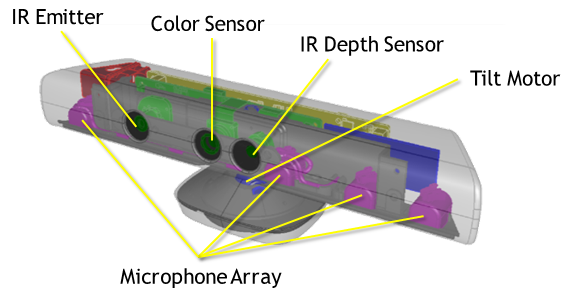
\includegraphics[width=90mm]{./figuras/kinectEstructura}
	\caption[Componentes internos del Kinect\textcopyright ]{Componentes internos del Kinect\textcopyright: IR Emitter: proyector de luz infrarroja; IR Depth Sensor: sensor CMOS monocromo estándar; Color Sensor: cámara RGB; Tilt Motor: Motor; Microphone Array: conjunto de 4 micrófonos \hyperlink{e06}{[E06]}} \label{fig:kinectEstructura}
\end{figure}
%de: https://msdn.microsoft.com/en-us/library/jj131033.aspx%
Para la detección y obtención de la información de la persona, se requiere de un dispositivo el cual nos proporcione todos los datos necesarios para facilitar el desarrollo del sistema. Para ello, se propuso el uso de un sensor de profundidad el cual nos brindará todo lo necesario para la fase de programación. Es por eso que se decidió utilizar un Kinect\textcopyright\ versión 1, debido a su bajo costo en el mercado y a que posee dicho sensor de profundidad, además de una cámara RGB la cual se podría utilizar en trabajo futuro para conseguir un modelo de detección mas robusto. Dicho esto, procedamos a conocerlo a detalle.\\
Kinect es un dispositivo originalmente dirigido a los juegos de la consola Xbox 360\textregistered, desarrollado por Microsoft\textregistered, el cual es capaz de a través de gestos, controlar e interactuar con la interfaz de la consola y los juegos en donde se requiera el uso de éste. Está conformado por los elementos mostrados en la Figura (\ref{fig:kinectEstructura}), en donde el sensor de profundidad, está formado por dos componentes: un proyector de luz infrarroja (IR Emitter) y un sensor CMOS monocromo estándar (IR Depth Sensor), los cuales se basan en un principio parecido al de triangulación entre los rayos visuales de los puntos proyectados y sus correspondientes proyecciones en la imagen; además posee una cámara RGB (Color Sensor), cuyo funcionamiento es igual a la de una cámara digital estándar. También tiene 4 micrófonos (Microphone Array) y un motor (Tilt Motor) que es utilizado para orientar el campo de visión de las cámaras. Cabe mencionar, que existen dos modelos para la versión 1 del kinect\textcopyright, uno conocida como kinect\textcopyright\ para Xbox 360, que para su uso en una computadora se requiere de un adaptador USB, mientras que existe un kinect\textcopyright\ para Windows, que aunque posee mejoras, su costo hoy en día es mucho mas elevado que la versión para la consola y es por ello que en ése trabajo de tesis se optó por el primero (proporcionado por la Universidad Veracruzana). Teniendo en cuenta ello, en la tabla \ref{tabla:especKinect}, se presentan las características principales del kinect\textcopyright\ para xbox 360.\\
\begin{table}[H]
	\centering
	\begin{tabular}{>{\centering\arraybackslash}m{6cm} >{\arraybackslash}m{7cm} }
		\hline
		Componentes & Características\\
		\hline \hline
		Cámaras: Profundidad y Color
		&
\begin{itemize}
	\item Resolución: 320x240 ó 640x480
	\item Campo de Visión: 43$^{\circ}$ vertical, 57$^{\circ}$ horizontal
	\item Velocidad de frames: 30 Frames por segundo (30 FPS)
	\item Distancia recomendada: entre 0.8m y 3.5 m
\end{itemize}	
		\\
		\hline
		Micrófonos & 
		\begin{itemize}
			\item Posee 4 micrófonos (ADC), con cancelación de eco acústico y supresión de ruido
			\item Frecuencia: 16-khz
			\item 24-bit mono modulación de código de pulso (PCM)
		\end{itemize}
		 \\
		\hline
		Motor &
		\begin{itemize}
			\item  Rango de inclinación: $ \pm $27$^{\circ}$ 
		\end{itemize}\\
		\hline
	\end{tabular}
	\caption{Especificaciones técnicas del Kinect para Xbox 360.}
	\label{tabla:especKinect}
\end{table}
\subsubsection{Proyector}
Debido a que éste trabajo de tesis es basado en la tecnología SAR, el uso de un proyector digital es indispensable para mostrar la información virtual. La calidad de éstos varía principalmente en el tipo de tecnología utilizada, modelo y distancia focal con el objetivo. A partir de ello, los elementos a tener en cuenta al momento de elegir un proyector son: tamaño de la imagen, resolución, luminosidad y contraste, tiempo de vida de la lámpara y el nivel sonoro. Enfocándonos en la luminosidad de un proyector, ésta es expresada en lúmenes y se puede definir como la medición de la emisión de color de un proyector. Mientras mayor sea su número, más vivo y real será la imagen, que es uno de los objetivos que se intenta conseguir en éste trabajo de tesis, por lo que para tener una experiencia de visionado satisfactorio se debe contar con un mínimo de 1600 lúmenes. Ahora, si el proyector de nuestra elección posee muchos lúmenes pero un contraste bajo, la imagen se mostrará descolorida, debido a que la cantidad de luz en la pantalla hace que el negro pierda intensidad. Partir de un nivel mínimo de 1.500:1 es lo recomendado.
\begin{figure}[htb]
	\centering
	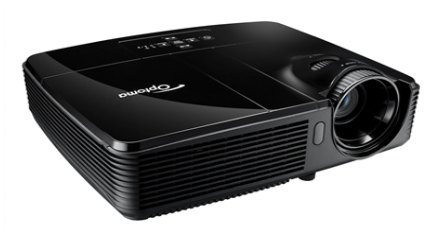
\includegraphics[width=70mm]{./figuras/proyector}
	\caption{Proyector Optoma DX551}\label{fig:proyector}
\end{figure}\\
Para la implementación se utilizará un proyector Optoma DX551 (Figura \ref{fig:proyector}) por parte de la Universidad Veracruzana con las siguientes especificaciones técnicas:
\begin{table}[H]
	\centering
	\begin{tabular}{>{\arraybackslash}m{6cm} >{ \arraybackslash}m{7cm} }
		\hline
		Componentes & Características\\
		\hline \hline
	 	Tecnología del display
		&
		Single 0.55" DMD DLP\textregistered
		\\
		\hline
		Luminosidad & 
		2800 ANSI Lúmenes
		\\
		\hline
		Contraste &
		3500:1\\
		\hline
		Tiempo de vida de la lámpara &
		5000 horas (normal); 6000 horas (eco)\\
		\hline
		Distancia de la proyección &
		1.2 a 12 metros\\
		\hline
		Resolución máxima  & 
		UXGA (1600 x 1200); 1080p (1920 x 1080)\\
		\hline
	\end{tabular}
	\caption{Especificaciones técnicas del Proyector Optoma DX551}
	\label{tabla:especProyector}
\end{table}
\paragraph{Lugar de proyección}
Para obtener buenos resultados de la imagen, es necesario tomar en cuenta el color y el material en donde será proyectado. En un inicio se había considerado proyectar la imagen encima de una mesa de color negro (éste tipo de proyección es considerada como front-projection que fue explicado en el capítulo anterior). Sin embargo, esta disposición del proyector, no permite que el observador se acerque mucho a la proyección, debido a que puede obstruir la imagen proyectada con su cabeza o manos. Como solución a ello, se decidirá utilizar la técnica de retroproyección (igual explicada en el capítulo anterior \hyperlink{e11}{[E11]}), la cual permitirá acercarse a la proyección sin la limitante anterior debido a que el proyector se encontrará debajo de una mesa (con material traslúcido o semi-traslúcido) y la imagen será proyectada de abajo hacia arriba, mostrando la información por la parte delantera (para una idea mas clara de lo explicado véase figura \ref{fig:disenoPre}, en donde se muestra el diseño preliminar del escenario de pruebas). El material ideal para este tipo de proyección es conocido como DNP Holoscreen, pero el precio es muy elevado (entre 200 y 500 dólares, dependiendo de su tamaño), por lo que se tiene pensado utilizar materiales semi-traslúcidos como papel o películas de plástico semitransparentes adheridas a un lámina de plástico transparente, en donde se pueda retener parte de la luz proyectada.\\
\subsubsection{Computadora}

Para determinar las características mínimas que se necesitan para que nuestro sistema funcione correctamente, se debe realizar un análisis previo del hardware y software que se utilizará. Después de dicho análisis, se determinó que una computadora con los siguientes requisitos mínimos no debería tener problemas en la ejecución del programa:
\begin{itemize}
	\item Procesador de 32 bits (x86) o 64 bits (x64)
	\item Procesador de doble núcleo, de 2.66-GHz o más rápido
	\item Bus USB 2.0 dedicado
	\item 2 GB de RAM
	\item Puerto VGA para proyector
\end{itemize}
\begin{figure}[htb]
	\centering
	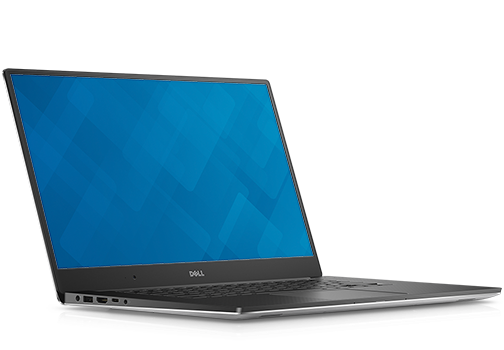
\includegraphics[width=70mm]{./figuras/dell}
	\caption{Dell Mobile Precision Workstation 5510}\label{fig:dell}
\end{figure}
La computadora en la cual se realizará el desarrollo y ejecución del sistema, será una Laptop Dell Mobile Precision Workstation 5510 (Figura \ref{fig:dell}), que cuenta con las siguientes especificaciones técnicas: 
\begin{table}[H]
	\centering
	\begin{tabular}{>{\arraybackslash}m{4cm} >{ \arraybackslash}m{9cm} }
		\hline
		Componentes & Características\\
		\hline \hline
		Procesador
		&
		Sexta generación del procesador Intel® Core™ i7-6820HQ (8MB Caché, hasta 3.60 GHz)
		\\
		\hline
		Memoria & 
		8GB de Memoria DDR4 a 2133MHz SDRAM, sin paridad [Non-ECC] (2 DIMMs)
		\\
		\hline
		Disco Duro &
		Disco de estado sólido (SSD) SATA de 256GB de 2.5"\\
		\hline
		Tarjeta de Video &
		NVIDIA® Quadro® M1000M con 2GB GDDR5\\
		\hline
	\end{tabular}
	\caption{Especificaciones técnicas de Laptop Dell Mobile Precision Workstation 5510}
	\label{tabla:especDell}
\end{table}
\subsection{Software del sistema}
En esta sección se analizará todo lo referente al software que se utilizará en el desarrollo e implementación del sistema, de tal modo que se pueda aprovechar al máximo los recursos hardware, y obtener resultados satisfactorios en el rendimiento, debido a que es un sistema que se ejecutará en tiempo real.
\subsubsection{Sistema Operativo}
El sistema operativo en donde se desarrollará el proyecto, será Ubuntu, específicamente la versión 16.04. Es una de las distribuciones Linux, que a diferencia de otros sistemas operativos es capaz de aprovechar mejor los recursos hardware, y que debido al bajo consumo que se requiere, la velocidad de procesamiento es mayor. Una de las ventajas y una de las razones por la cual se utiliza éste Sistema Operativo, es debido a que cuenta con el paquete de python 2.7 (por defecto) instalado (que será el lenguaje de programación que se utilizará), lo cual facilita el uso del mismo a través de la terminal, además de que la instalación de las librerías y conexión con el kinect\textcopyright\ se obtienen de una manera sencilla a través de pocos comandos. 
\subsubsection{Python}
Python es un lenguaje de programación interpretado multiparadigma y multiplataforma y será el que se utilizará para el desarrollo del sistema. Muchas de las ventajas que nos ofrece son su facilidad de uso, portabilidad, legibilidad y simplicidad. Fue diseñado principalmente para expresar en forma clara y directa instrucciones que debe seguir un programa, sin la necesidad de estar indicando los detalles de bajo nivel los cuales involucran los tipos de variables, sus tamaños y manejo de memoria, y es por ello que se le denomina intérprete, debido a que es capaz de inferir esos detalles. Lamentablemente esas ventajas tienen su costo, debido a que se ejecuta mas lento que otros lenguajes tradicionales (por ejemplo los compilados, que son ejecutados directamente por el procesador). A pesar de ello, cada vez existen mas librerías (tales como numpy, math, opencv (utilizadas en el desarrollo)) y herramientas de apoyo que agilizan algunos procesos que son mas lentos si son desarrollados directamente en este lenguaje, lo cual convierte a python en un lenguaje potente actualmente. 
\subsubsection{LibFreenect}
Casi inmediatamente con la aparición del Kinect\textcopyright\ en el mercado, y debido a su facilidad de adquisición (precio muy bajo en comparación con otros sensores), muchas fuentes alternas a través de ingeniería inversa lograron desarrollar controladores que permitían acceder a la información tanto de la cámara RGB como la de profundidad, convirtiéndose entonces en un sistema de visión artificial muy utilizado por investigadores, que incluso Microsoft\textregistered\ un tiempo después decidió lanzar un SDK (Software Development Kit) para desarrollo investigativo, pero dirigido a su sistema operativo y utilizando c\# como lenguaje de programación.\\
OpenKinect es una comunidad abierta, que distribuyen utilidades y aplicaciones para el Kinect\textcopyright, y que ha sido de gran ayuda para el desarrollo de éste sistema. La librería en donde se encuentran todos los drivers, funciones y ejemplos es libfreenect, y está disponible para muchos sistemas operativos (entre ellos Ubuntu), es fácil su instalación y uso, por lo que éste será el medio con el que nos comunicaremos con Kinect\textcopyright.
\subsubsection{OpenCV}
OpenCV (Open Source Computer Vision Library) es un librería que ha sido de gran utilidad en el área de la visión por computadora. Debido a que python será el lenguaje utilizado, el uso de ésta optimizará y agilizará el proceso de análisis y procesamiento de imágenes, lo cual es una gran ventaja debido a que el proceso se realiza en tiempo real. La versión que viene por defecto al momento de instalarlo es (2.4.9.1), y se utilizará en gran medida para el tratamiento de las imágenes (aplicando filtros) y detección de figuras a través de técnicas de visión artificial, en conjunto con otra librería muy utilizada (numpy), que nos ayudará mayormente para operaciones con matrices.
\subsubsection{Blender}
La información virtual que se mostrará en nuestro entorno, será diseñada a través de Blender. Éste es un programa multiplataforma que se puede utilizar como modelado, animación y creación de gráficos en 3D. De igual manera, posee un motor de juegos interno, lo cual abre la posibilidad de que en futuro se pueda agregar una fase de interacción entre los elementos virtuales y el usuario. Es distribuido de forma gratuita y es compatible con Ubuntu. Además, el uso de la cámara virtual en blender nos proporciona el campo de vista que el observador debería tener, habiendo entonces una equivalencia real entre la cámara y la persona detectada. Cuenta con la creación de scripts en python para automatizar y manipular los objetos (pero la versión 3, lo cual tiene algunas diferencias con la 2.7). La versión de blender que se utilizará será la 2.76.
\section{Diseño General del Sistema}
Después de un análisis detallado de los elementos que estarán involucrados en el desarrollo del sistema, se determinó como diseño general el siguiente esquema (Figura \ref{fig:esquemaGeneral}), el cual se realizó para definir las etapas por las cuales tendrá que seguir el sistema cada vez que se capture una imagen (frame) a través de un sensor de profundidad (en éste caso el kinect\textcopyright\ de Microsoft\textcopyright, descrito en la sección anterior). Este análisis fue basado en la premisa de que para obtener la perspectiva de un persona correspondiente a un escenario 3D, se debe determinar primero si se encuentra una persona en el entorno, para así conocer la información respecto a ésta (es decir su posición y altura), y así poder proyectar los elementos virtuales en relación con el observador.\\
\begin{figure}[tbh]
	\centering
	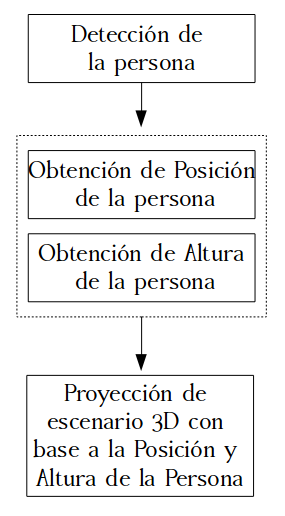
\includegraphics[width=60mm]{./figuras/esquemaGeneral}
	\caption[Esquema general del sistema]{Esquema general del sistema: Módulos por los que tendrá que seguir el sistema de manera subsecuente  para su funcionamiento} \label{fig:esquemaGeneral}
\end{figure}
Se siguió el patrón de desarrollo de software conocido como modelo incremental (o iterativo), que es una mejora del modelo tradicional de cascada, el cual consiste en la secuencia de las etapas del tradicional (análisis, diseño,  implementación y pruebas) pero de una manera superficial, el cual se utiliza mayormente para obtener resultados a corto plazo del software (a veces se pueden obtener prototipos funcionales por varios incrementos), con la posibilidad de agregar o quitar funcionalidades conforme vaya avanzando el sistema, para obtener mejores resultados en cada uno de los módulos. Dicho esto, como primera fase o prototipo 1, se diseñó el sistema detectando a la persona de forma manual (mas adelante se explicará ésto), basándose únicamente en la posición de la persona (sin tomar en cuenta su altura), lo cual daría como resultado, que el escenario se adaptara a la posición de la persona rotando en el eje vertical, sin variar el ángulo de inclinación entre la proyección y el observador. Una vez implementado esta fase, pasaríamos a la siguiente o prototipo 2, el cual incluirá la detección automática y la obtención de la altura de la persona basado en la información de la imagen de profundidad para la obtención correcta de la perspectiva de la persona.
\subsection{Prototipo 1}
\begin{figure}[th]
	\centering
	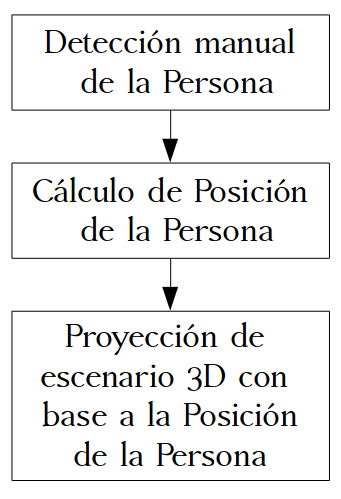
\includegraphics[width=55mm]{./figuras/proto1}
	\caption[Esquema general de prototipo 1]{Esquema general de prototipo 1: Pasos que se seguirán para proyectar el escenario 3D con base en la posición} \label{fig:proto1}
\end{figure}
Como fase inicial, este prototipo será la base para mejoras futuras, por lo que debe tener un diseño claro y bien estructurado, para evitar problemas en su funcionamiento a largo plazo. Constará con un fase inicial de detección, la cual denominaremos detección manual debido a que se ajustará el umbral de detección de forma manual; ademas se diseñará el módulo para obtener la posición de la persona y el módulo para proyectar el escenario 3D con base en su posición (Figura \ref{fig:proto1})

\subsubsection{Detección manual}
Como fue mencionado anteriormente, el diseño inicial de detección de la persona se basará dependiendo del umbral asignado por el usuario. Es decir, la imagen de profundidad será obtenida por el kinect\textcopyright\ en la escala de grises, se binarizará a través de un umbral dado por el usuario que delimitará el fondo de la persona para poder obtener su contorno. Debido a que el sensor de profundidad se encontrará a una distancia aproximada de 2.90 metros del suelo, capturando entonces la información desde arriba, el contorno que necesitaremos será el de la cabeza de la persona. El esquema general que muestra los pasos para éste módulo lo podemos encontrar en la Figura \ref{fig:deteccManual}.
\begin{figure}[th]
	\centering
	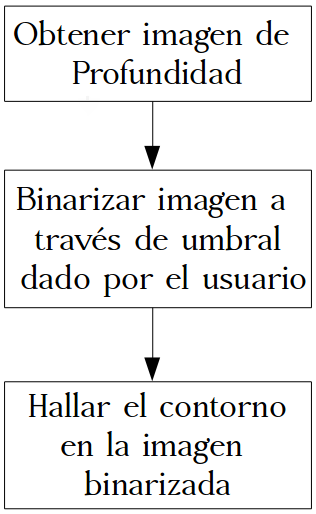
\includegraphics[width=60mm]{./figuras/deteccionManual}
	\caption[Esquema general de detección del prototipo 1]{Esquema general de detección del prototipo 1: Instrucciones básicas para el módulo de detecció manual} \label{fig:deteccManual}
\end{figure}
\subsubsection{Posición de la Persona}
Para calcular la posición de la persona, se determinó que a través de la figura generada del contorno de ésta, se hallaría el punto central, lo cual, en otras palabras nos daría la posición del pixel en la imagen, en un rango de 640x480 (tamaño de la imagen), en donde ésta información se almacenará en un archivo para que se pueda obtener en el motor de juegos que se utilizará (Blender). Para poder llegar a éste módulo, es necesario que se haya detectado la persona en la etapa anterior, de lo contrario, si no se obtiene un contorno, no se puede determinar la posición, y el programa se detendría. En la figura \ref{fig:posicion} se muestran los pasos para determinar la posición de la persona.
\begin{figure}[th]
	\centering
	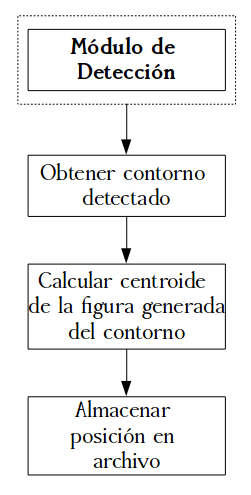
\includegraphics[width=60mm]{./figuras/posicion}
	\caption[Esquema general de posición del prototipo 1]{Esquema general de posición del prototipo 1: serie de pasos que se seguirán para poder detectar la posición central del contorno detectado} \label{fig:posicion}
\end{figure}
\subsubsection{Proyección con base en la Posición}
Éste módulo, se encuentra internamente en el programa Blender, y es el encargado de posicionar la cámara virtual, en la posición obtenida del archivo. El escenario recreado poseerá las mismas medidas que el de la cámara depth 640x480, pero una cifra menos (es decir 64.0x48.0) debido a la gran expansión que ocasionaría si se utilizaran las dimensiones originales. De éste modo, al obtener la posición de la persona, la posición de la cámara será las coordenadas serán divididas entre diez. Es importante recalcar, que aunque la cámara y la posición de la persona, serán equivalentes, al momento de posicionar la cámara virtual, ésta mantendrá los mismos ángulos que enfocan a un determinado punto, por lo cual será necesario dirigir el campo de vista de ésta hacia el centro del escenario calculando sus respectivos ángulos. En la figura \ref{fig:proyeccionProto1}  podemos ver los pasos para llegar al objetivo final.
\begin{figure}[th]
	\centering
	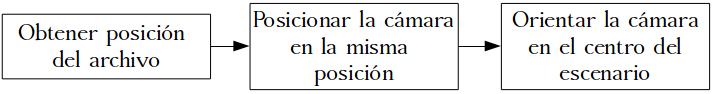
\includegraphics[width=55mm]{./figuras/proyeccionProto1}
	\caption{Esquema general de proyección del prototipo 1} \label{fig:proyeccionProto1}
\end{figure}
\subsection{Prototipo 2}
Después de obtener un prototipo funcional, se incluirá a través de varias mejoras un prototipo 2, el cual involucre la optimización de la detección de la persona, logrando que se realice de manera automática y la adición del módulo de la altura, lo cual implicaría modificar un poco la parte de proyección en blender y sus ángulos en la cámara. Lo anterior se puede resumir en la figura \ref{fig:proto2}, en donde se definen cada una de las etapas que se analizarán a continuación.
\begin{figure}[th]
	\centering
	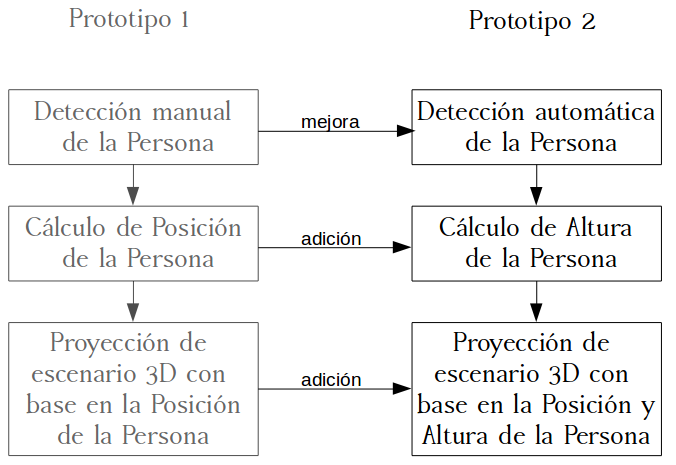
\includegraphics[width=150mm]{./figuras/proto2}
	\caption{Esquema general de prototipo 2} \label{fig:proto2}
\end{figure}

\subsubsection{Detección automática}
Basado en los pasos definidos en el módulo de detección manual (donde para detectar el contorno de la cabeza de la persona se ajusta el umbral por el mismo usuario dependiendo de la altura de éste), se diseña un modelo de detección capaz de ajustar éste umbral de manera automática, basado en un rango de área permitida. Es decir, si el umbral es muy elevado, el contorno detectado estará involucrando más allá del área de la cabeza de la persona (por ejemplo los hombros) dando como resultado que el cálculo de la posición podría verse afectada. Por lo tanto, se define un intervalo de área mínima y máxima permitida, calculada a través de un rectángulo delimitador que contendrá el contorno (esto para dar un poco mas de libertad en la forma de los contornos detectados), y dependiendo del área calculada del rectángulo delimitador con el umbral actual, se irá ajustando éste umbral hasta que el área actual se encuentre dentro del rango definido. Al tomar en cuenta esto, el umbral se ajusta de manera automática, de tal modo que si una persona es de mayor o menor altura, detectará la región de la cabeza siempre, y aunque varíe su altura (se incline o agache) en el transcurso de la detección, siempre se seguirá el área de la cabeza, algo que en el módulo anterior no se podía realizar. En la figura \ref{fig:deteccAutomatica}, se muestra un esquema de cómo se realizaría ésta etapa del sistema.
\begin{figure}[th]
	\centering
	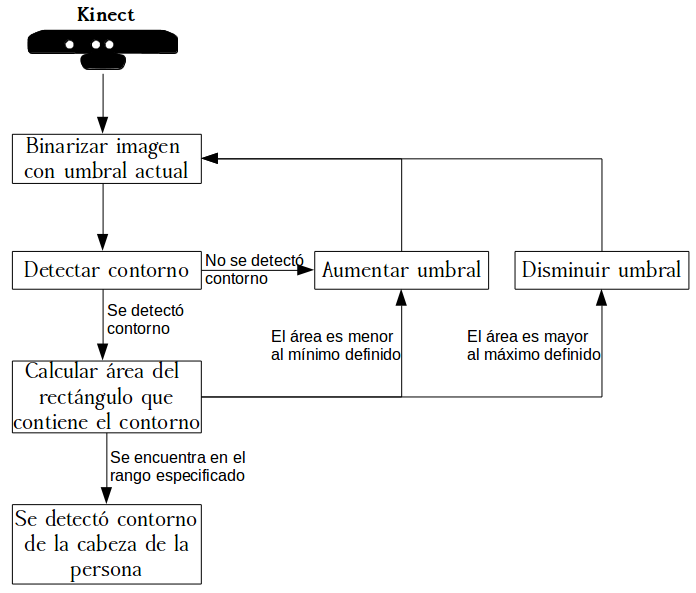
\includegraphics[width=150mm]{./figuras/deteccionAutomatica}
	\caption{Esquema general de detección automática} \label{fig:deteccAutomatica}
\end{figure}
\subsubsection{Altura de la Persona}
Éste tal vez sea el módulo mas rápido y fácil de implementar. Debido a que la detección automática ajusta el umbral para obtener el contorno de la cabeza de la persona y luego es obtenida la posición a través el centro del contorno, el cual se puede interpretar como la posición en píxeles de la imagen, la altura entonces es determinada por el valor de la imagen de profundidad en el punto proporcionado por el módulo de posición. Por lo tanto, éste módulo podría encontrarse dentro del módulo de posición y almacenar la información en un archivo como coordenadas en un espacio 3D, para su posterior uso en el módulo de proyección.
\subsubsection{Proyección con base en la Altura y Posición}
En lo que respecta a éste módulo, al adicionar la fase de detección de la altura de la persona, se debe hacer una equivalencia en el eje vertical de la cámara en blender con el valor dado por la imagen de profundidad. Una vez realizado el paso anterior, se orienta la cámara, es decir se inclina enfocando al centro del escenario (ésto se verá en detalle en la fase de implementación). En la figura \ref{fig:proyeccionProto2} se muestra un resumen de lo explicado anteriormente.
\begin{figure}[th]
	\centering
	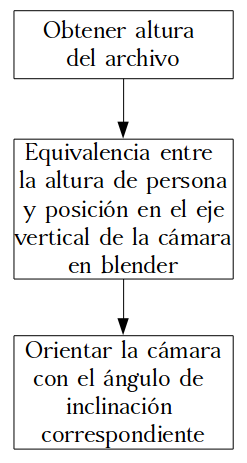
\includegraphics[width=50mm]{./figuras/proyeccionProto2}
	\caption{Esquema general de proyección de prototipo 2} \label{fig:proyeccionProto2}
\end{figure}
\subsection{Diseño preliminar de escenario}
Considerando que se utilizará la técnica de retroproyección (explicada anteriormente), se propuso entonces, como diseño previo del escenario un área que constará de un proyector que se localizará en la parte inferior de una mesa especial fabricada (debido a que en la superficie se utilizará un material especial (semi-traslúcido) para la retroproyección), un sensor de profundidad (Kinect\textcopyright) que se ubicará en el techo (visión aérea) de tal modo que podamos obtener una gran área lo mas libre de objetos posible y ubicar la mesa en el centro de detección para así darle la posibilidad al observador de abarcar todos los ángulos del escenario 3D proyectado, es decir, que se pueda caminar alrededor de ésta, pudiendo abarcar todo el campo de visión (360$^{\circ}$ en torno a ésta). Para que tengamos una idea mas clara de lo explicado, en la figura \ref{fig:disenoPre}  se muestra un diseño preliminar del escenario de pruebas.
\begin{figure}[th]
	\centering
	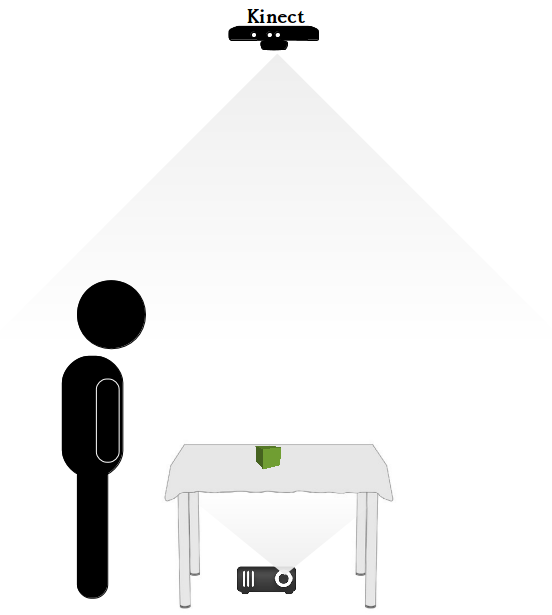
\includegraphics[width=110mm]{./figuras/disenoPre}
	\caption{Diseño preliminar del escenario de pruebas} \label{fig:disenoPre}
\end{figure}
\subsection{Funcionamiento del Sistema General}
\begin{figure}[th]
	\centering
	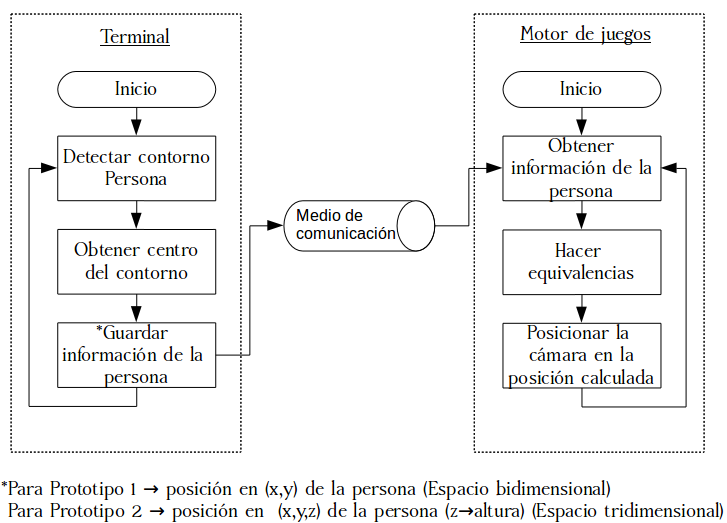
\includegraphics[width=150mm]{./figuras/sistemaGeneral}
	\caption[Funcionamento del Sistema General]{Funcionamento del Sistema General: Funciones principales que intervendrán en el proceso de ejecución.} \label{fig:sistemaGeneral}
\end{figure}
De acuerdo a lo explicado anteriormente y para tener una idea mas clara de como se comportará el sistema, en la figura \ref{fig:sistemaGeneral} se muestra una representación de las funciones principales que intervendrán en el sistema general. Podemos entonces definir que será dividido en dos grandes subsistemas que se ejecutarán al mismo tiempo y que la forma en la que se estarán comunicando será a través de un archivo de texto llamado infoPersona.txt. Éste contendrá la información necesaria para que el subsistema por parte de blender, sea capaz de posicionar la cámara virtual dependiendo de la última modificación del archivo por parte del subsistema de la terminal. El uso del archivo nos beneficia en caso de si el subsistema de la Terminal falla, el otro subsistema no se detendría debido a que usaría la última posición modificada, y así la información proyectada no finalizaría, solo quedaría estática. En cuanto al contenido del archivo, su información dependerá del prototipo en donde nos encontremos, es decir, para el prototipo 1, se manejaría únicamente las coordenadas (x,y) de la imagen, siendo entonces un espacio bidimensional (2 variables involucradas), mientras que en el prototipo 2, se agregaría una variable más (la altura), lo cual estaríamos hablando de un espacio de 3 dimensiones (x,y,z).
%%%%%%%%%%%%%%%%%%%%%%%%%%%%%%%%%%%%%%%%%%%%%%%%%%%%%%%

%%%CAPÍTULO 4 -> IMPLEMENTACIÓN Y RESULTADOS%%%

\chapter{Implementación y resultados}\label{cap.implementacionyresultados}
\fancyhead[R]{CAPÍTULO 4. IMPLEMENTACIÓN} 
Luego de analizar, definir los requerimientos del sistema, realizar el diseño y esquematización, pasamos a la etapa de implementación. Se abordará a detalle el proceso de desarrollo, así como los resultados generados en cada uno de los prototipos propuestos con el objetivo de identificar errores, proponer soluciones a los problemas y optimizar cada uno de los módulos.\\
A partir de los módulos identificados en el capítulo anterior, siguiendo los principios de programación orientada a objetos, con el objetivo que se puedan agregar funcionalidades y mejorar sus métodos por separado, el sistema fue desarrollado a través de clases las cuales son: Detección, Posición y Persona. El módulo de Proyección se encuentra embebido en el programa blender, por lo cual no se desarrolló como clase y el módulo de Altura se encontrará en la clase Posición, debido a su fácil adquisición a través de los resultados de los demás módulos y por lo tanto no será necesario definir una clase para ella. La clase Persona, es necesaria debido a que será el medio en el que se comunicarán las demás clases del subsistema de Terminal; además, tener un clase que tenga la información de un persona fue pensado para que en trabajo futuro se pudiese hacer seguimiento de varias personas teniendo un registro de la posición de cada una de ellas e ir alternando la perspectiva conforme lo requieran. En la figura \ref{fig:diagramaClases} se muestra el diagrama de clases que define la estructura del subsistema de Terminal, con sus atributos y métodos de cada una de las clases (Detección, Posición y Persona) dependiendo del prototipo en donde nos encontremos. El subsistema por parte de Blender, sólo tendrá el módulo de Proyección en un script embebido en éste.\\

\begin{figure}[th]
	\centering
	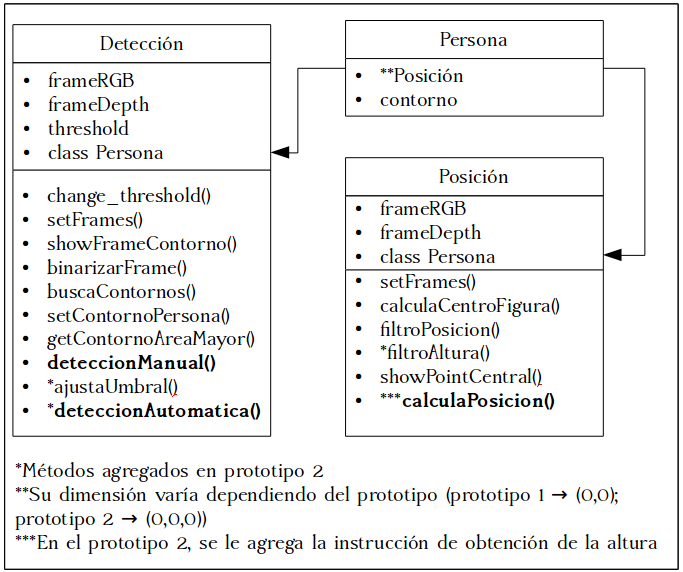
\includegraphics[width=140mm]{./figuras/diagramaClases}
	\caption{Diagrama de clases de subsistema de Terminal} \label{fig:diagramaClases}
\end{figure}

\section{Escenario de pruebas}
\begin{figure}[ht]
	\centering
	\hspace{-2mm}
	\subfigure[Parte frontal de la mesa]{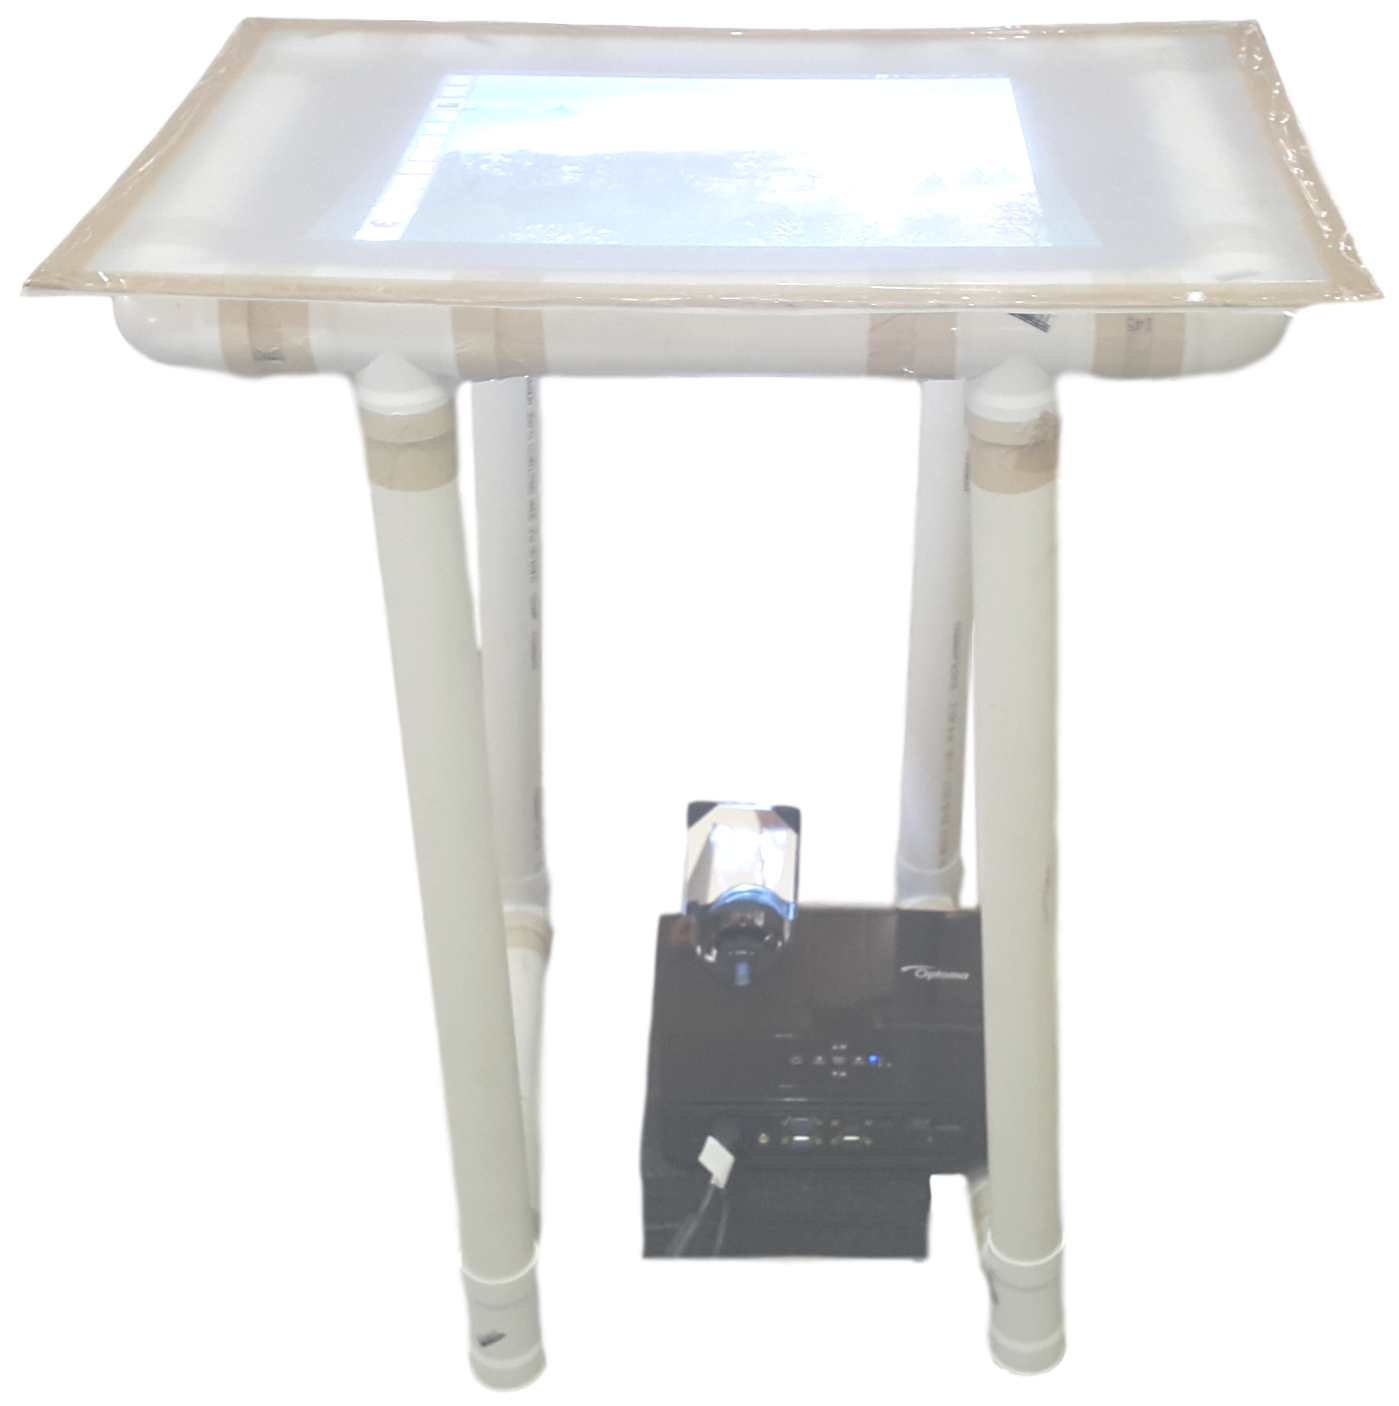
\includegraphics[width=52mm]{./figuras/mesa1}}
	\hspace*{10mm}
	\subfigure[Parte lateral de la mesa]{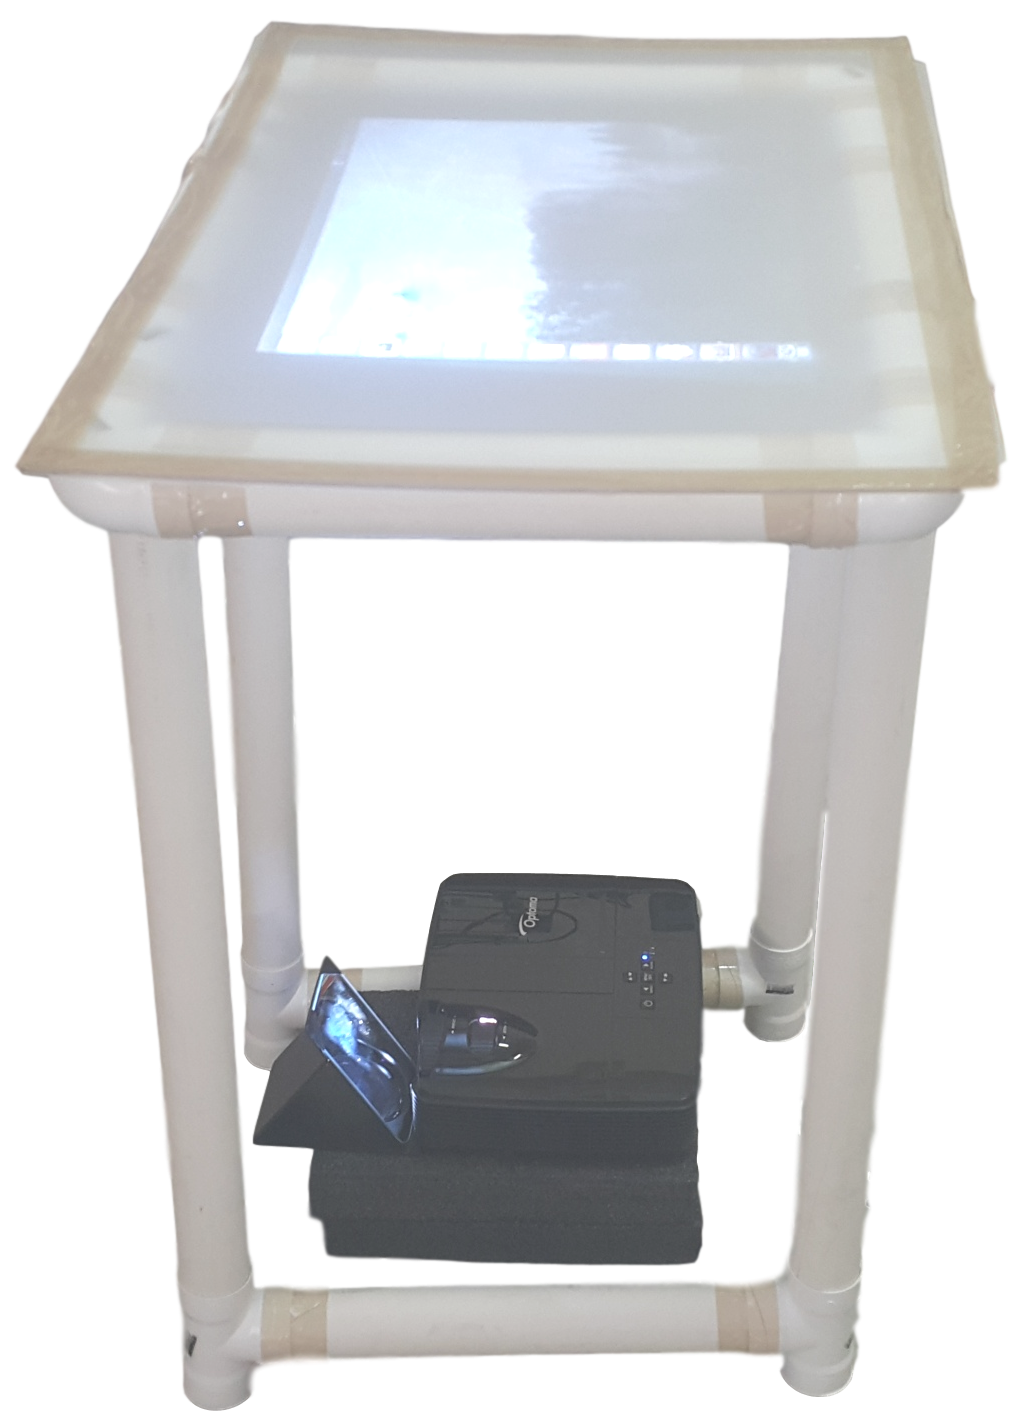
\includegraphics[width=40mm]{./figuras/mesa2}}
	\caption{Mesa donde se realizará la retroproyección} \label{fig:mesa}
\end{figure}
Después de haber realizado un diseño preliminar del escenario en donde se mostrará la información virtual, y decidir que se utilizará la técnica de retroproyección, se determinó que la manera mas asequible y fácil de contruir una mesa sería a través de tubos pvc, de tal modo que se pudiera poner encima de ella (como base), el material que retendrá la luz proyectada para ser mostrada en la parte superior. Se utilizó una lámina de plástico policril transparente, y adherida a ésta una película de plástico texturizado, que ayudó en gran medida a retener la proyección (Figura \ref{fig:mesa}). En la parte inferior, se encontrará el proyector, que con el objetivo de aumentar la imagen, se utilizó un espejo frente a éste, que entonces será el que reflejará la imagen en la parte superior.


\section{Prototipo 1}
Como primera fase de desarrollo, y de acuerdo con el esquema general de este prototipo diseñado en el capítulo anterior, la figura \ref{fig:mainProto1}, muestra el diagrama de flujo que representa la función principal o base por parte del subsistema de Terminal, en donde se encuentran los métodos de las clases que intervendrán en el proceso de ejecución del sistema. De esta manera, podemos ver que se ejecuta siempre y cuando el kinect\textcopyright\ se encuentre conectado. En dicho caso, se puede acceder a la información y proceder con los siguientes métodos de las clases (Detección y Posición), para que de éste modo se pueda almacenar la información en un archivo de texto (infoPersona.txt) el cual es la conexión entre los dos subsistemas. Dicho esto, se explicará a continuación los métodos principales que intervienen en el funcionamiento de éste prototipo, que son Detección Manual y Posición (Calcular Posición), así como el módulo de Proyección que se encuentra embebido en Blender y es el que conforma nuestro segundo subsistema.
\begin{figure}[ht]
	\centering
	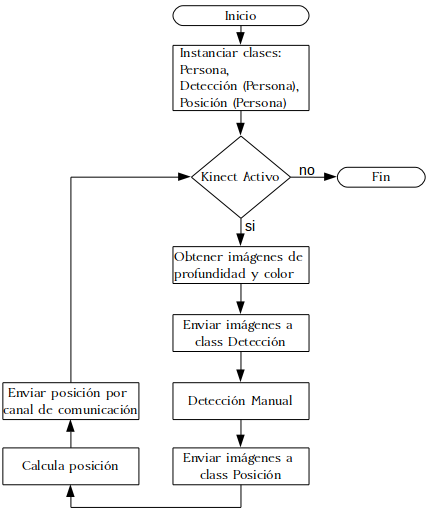
\includegraphics[width=120mm]{./figuras/mainProto1}
	\caption{Diagrama de flujo: función Principal de prototipo 1} \label{fig:mainProto1}
\end{figure}
\subsection{Detección manual}
Como se pudo observar en el diagrama de clases (Figura \ref{fig:diagramaClases}), dentro de la clase Detección, se define un método llamado ``deteccionManual()'', siendo éste el método de detección en éste prototipo encargado de realizar la función de buscar el contorno de la persona variando el umbral de forma manual con el objetivo de delimitar el fondo de la persona.\\
Debido al sensor y a la versión utilizada para la adquisición de la imagen de profundidad, la información obtenida es sensible y propensa a ruidos en la imagen capturada. Es por ello que el uso de filtros en la imagen (principalmente de suavizado o desenfoque(blur)) pueden ayudar a que la detección del contorno no varíe demasiado. Esto lo podemos ver en la figura \ref{fig:filtrado}(a), en donde se muestra una secuencia de imágenes de profundidad sin previo tratamiento de una persona que no se movió en un segundo. Para ello, uno de los filtros mas utilizados para desenfocar o suavizar una imagen es el conocido como Gaussian blur (desenfoque gaussiano), que se basa en aplicar un kernel Gaussiano sobre la imagen para así desenfocarla (ésta función es proporcionada por la librería openCV, en donde tenemos que especificar el tamaño del kernel (se propuso 5x5)) y fue el filtro que se utilizó para eliminar el ruido en torno al contorno de la persona. En la figura \ref{fig:filtrado}(b) se muestra entonces la prueba anterior, pero en este caso utilizando filtro.
\begin{figure}[ht]
	\centering
	\subfigure[Secuencia de imágenes de profundidad sin filtro capturadas en un segundo]{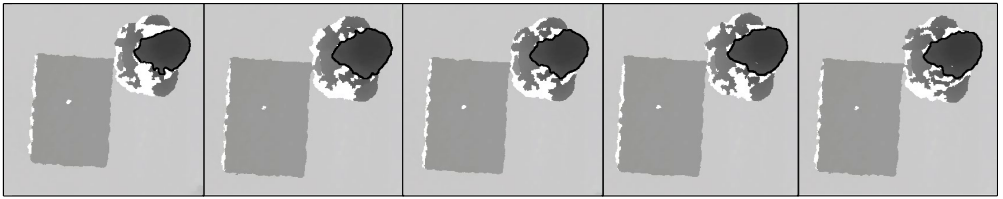
\includegraphics[width=140mm]{./figuras/sinBlur}}
	\subfigure[Secuencia de imágenes de profundidad con filtro capturadas en un segundo]{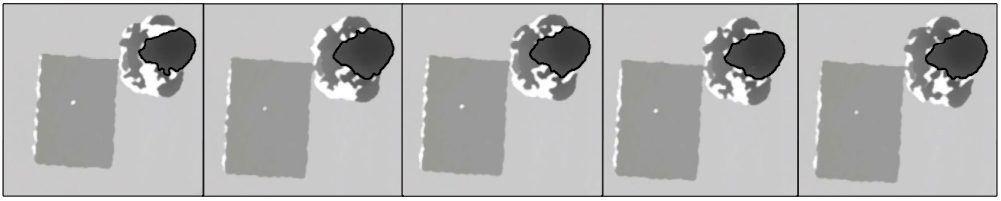
\includegraphics[width=140mm]{./figuras/conBlur}}
	\caption[Secuencia de imágenes de profundidad en un segundo sin filtro y con filtro]{Secuencia de imágenes de profundidad en un segundo sin filtro y con filtro: en la secuencia (a) se encuentran las imágenes sin tratamiento, mientras que la serie (b) se puede notar un suavizado (más en la última) de la misma secuencia, aplicando kernel Gaussiano.} \label{fig:filtrado}
\end{figure}\\
Pero, ¿cómo se determinará entonces el contorno? Luego del filtrado de la imagen, dependiendo del umbral establecido por el usuario (0 - 255 (que son los valores de profundidad que se pueden obtener)), se binarizará la imagen, es decir, se analizará toda la imagen (pixel por pixel) y con el valor asignado de umbral actual se determina si el pixel es blanco (255) o negro(0), por lo que la imagen mostrará una figura blanca que representará la cabeza de la persona en un fondo negro (éste método se encuentra igual dentro de la librería openCV) y en la figura \ref{fig:binarizacion} se puede ver una secuencia de 3 imágenes capturadas en un segundo que muestran la binarización explicada hace un momento. Terminado este proceso, se determinará entonces el contorno de la figura en blanco, a través de una una función que retorna una lista de los contornos en la imagen proporcionada igual por openCV. Debido al ruido que puede ocasionar el sensor (aún utilizando filtrado), se pueden llegar a detectar pequeños contornos que provoquen una detección errónea, por lo que se supone que el contorno de área mayor sea el de la persona y es seleccionado y almacenado como atributo en la clase Persona para su posterior uso. En la figura \ref{fig:diagFlujDeteccionManual} , se muestra un diagrama de flujo que de forma general resume lo explicado anteriormente.
\begin{figure}[ht]
	\centering
	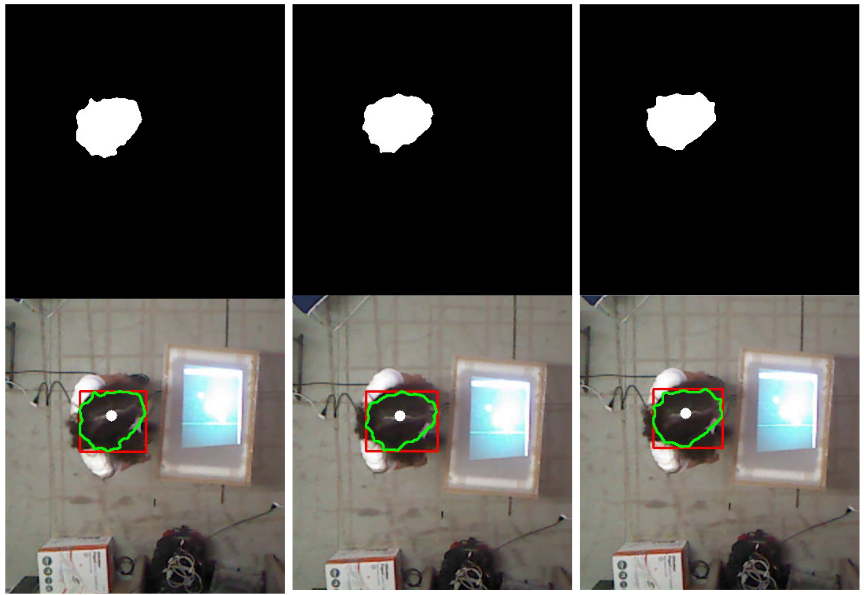
\includegraphics[width=120mm]{./figuras/binarizacion}
	\caption[Secuencia de imágenes de profundidad binarizadas y de imágenes RGB en un segundo]{Secuencia de imágenes de profundidad binarizadas y de imágenes RGB con el contorno de la cabeza detectado en un segundo} \label{fig:binarizacion}
\end{figure}
\begin{figure}[ht]
	\centering
	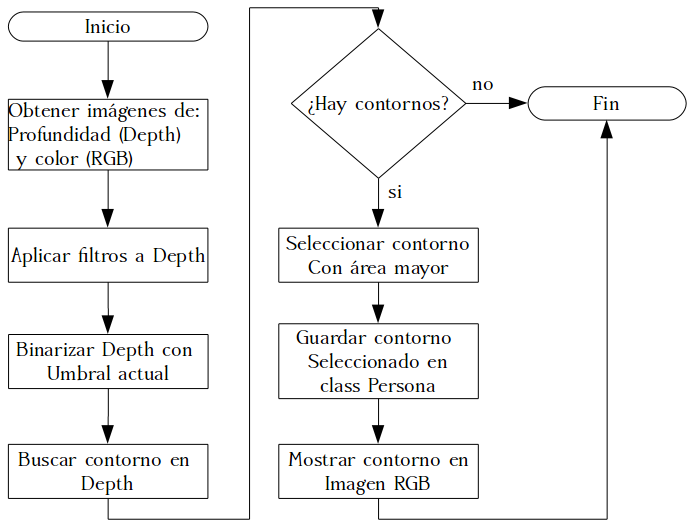
\includegraphics[width=130mm]{./figuras/diagFlujDeteccionManual}
	\caption{Diagrama de flujo de detección manual} \label{fig:diagFlujDeteccionManual}
\end{figure}
\subsection{Cálculo de la posición}
Luego de detectar e identificar el contorno de la persona, procedemos al cálculo de su posición. Para ello, lo primero es adquirir el contorno a través de la clase Persona el cual fue modificado en el método anterior (detección manual). La posición de la persona será determinada obteniendo el punto central del contorno, a través de Momentos de la Imagen. Éstos nos ayudan a obtener características de una imagen u objeto seleccionado (en nuestro caso, la figura que forma el contorno) tales como su área, perímetro y centro de masa del objeto (todo ello se puede obtener a través de una función dentro la librería openCV). En éste caso, lo que requerimos es el centro de la figura (centroide), que se puede obtener de la relación, $C_x = \frac{M_{10}}{M_{00}}$ y $C_y = \frac{M_{01}}{M_{00}}$.  Con ésto, obtenemos entonces el punto central, que varía dependiendo de la forma obtenida del contorno en la etapa anterior, sin embargo, a pesar de aplicar filtros para que no varíe mucho la forma, sigue existiendo un margen de error, lo cual ocasiona que la posición varíe unos cuantos píxeles al estar el observador quieto, por lo que se aplicó un filtro donde se toma en cuenta la posición analizada del frame anterior con la actual y se calcula la distancia en línea recta (distancia euclideana) entre estos dos valores suponiendo que en un rango (en éste caso de 5 píxeles), puede significar que la persona se encuentra en la misma posición y la variación es causada por parte del ruido ocasionado por el sensor. Una vez realizado éste paso, y dependiendo del resultado obtenido, se guardará la posición en el atributo de la clase persona, que en este caso será un vector de 2 posiciones, es decir $ (x,y) $. Para tener una idea general de lo explicado, véase figura \ref{fig:diagFlujPosicion}.
\begin{figure}[ht]
	\centering
	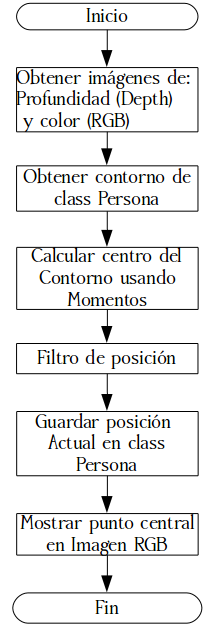
\includegraphics[width=40mm]{./figuras/diagFlujPosicion}
	\caption{Diagrama de flujo de Posición} \label{fig:diagFlujPosicion}
\end{figure}
\subsection{Proyección basada en la posición (x,y)}
Con respecto al subsistema por parte de blender, tenemos el módulo Proyección que ha sido analizado y diseñado anteriormente. Debido a que no existe forma de acceder a la interfaz y propiedades de Blender de manera externa (por Terminal), éste módulo se encuentra embebido en él. Es por ello, que para que el sistema general funcione, se requiere la ejecución paralela de los dos subsistemas. Se debe tener en cuenta que a pesar de que se encuentra python dentro de Blender, la versión por defecto que se utiliza es la 3.5.2, la cual varía un poco en algunas funciones, y fue necesario instalar las librerías numpy y math para ésta versión que permiten hacer los cálculos necesarios en éste subsistema.\\
\begin{figure}[htb]
	\centering
	\subfigure[Coordenadas de una imagen]{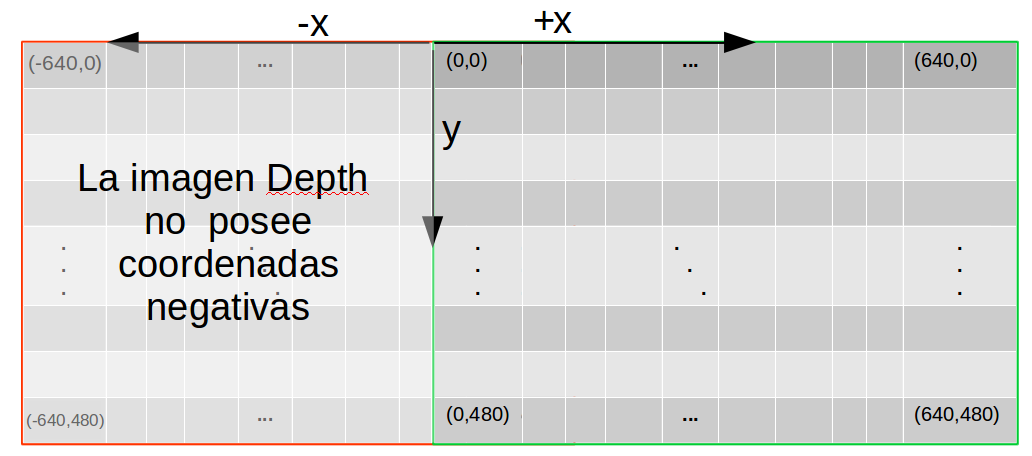
\includegraphics[width=120mm]{./figuras/coordsImagen}}
	\subfigure[Coordenadas en Blender]{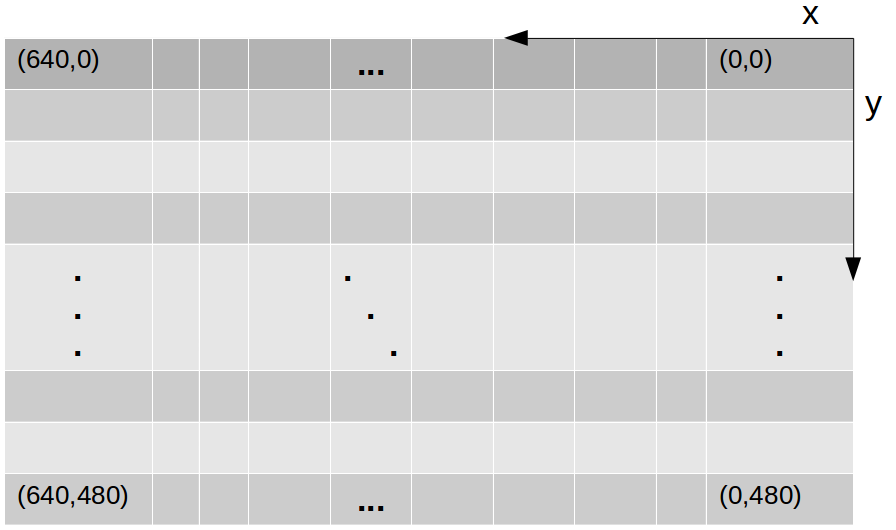
\includegraphics[width=118mm]{./figuras/coordsBlender}}
	\caption[Ejes de coordenadas en Imagen Depth y en Blender]{Ejes de coordenadas en Imagen Depth y en Blender ; En (b) entonces se manejará el eje de las x negativo para tener un correcta correspondencia con las coordenadas de la imagen} \label{fig:coords}
\end{figure}

\begin{figure}[thb]
	\centering
	\vspace*{5mm}
	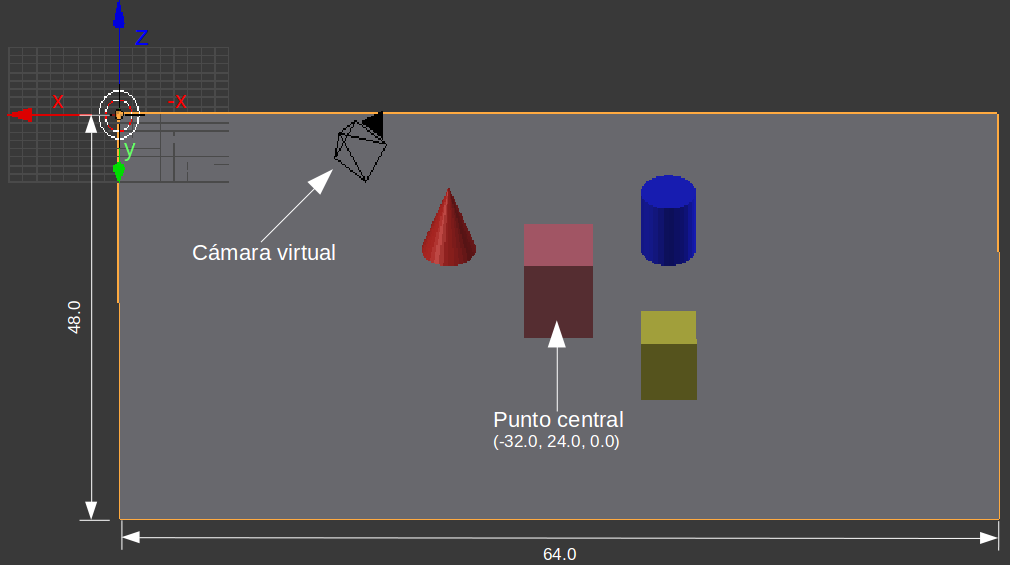
\includegraphics[width=120mm]{./figuras/escenarioBlender}
	\caption[Escenario virtual en Blender]{Escenario virtual en Blender; como puede notar en los ejes, el escenario se encuentra en el sentido positivo de las ordenadas, mientras que en el eje de las abscisas se encuentra en el sentido negativo} \label{fig:escenarioBlender}
\end{figure}

Para que existiera una equivalencia real, entre nuestro entorno y el entorno virtual, en un inicio se había decidido recrear el escenario virtual con las mismas dimensiones que la imagen de profundidad tiene como resolución (640x480), pero debido al gran número de coordenadas que generaría y por lo tanto un proceso mas lento de renderización, se decidió definir éste escenario con un tamaño diez veces menor (64.0x48.0), en donde los decimales serán el equivalente de la primera cifra (las unidades) de la imagen de profundidad, es decir, si tenemos una posición que se encuentra en el pixel (128, 264), el equivalente en blender de la posición será (-12.8, 26.4). Como se habrá dado cuenta, ésta última coordenada mencionada (la usada en blender), tiene el eje de las x como negativo, ésto debido a que las coordenadas en una imagen se encuentran como se muestra en la figura  \ref{fig:coords}(a) , mientras que en un sistema de coordenadas como el de blender, si el eje de las abscisas la consideramos como positiva se mostraría la proyección en espejo (Véase la diferencia de los sistemas de coordenadas en la misma figura \ref{fig:coords}), es por ello que al realizar la equivalencia de la posición también se necesita pasar el eje de las x a negativo para su correcta proyección. La figura \ref{fig:escenarioBlender} muestra el escenario en blender en donde nos podemos dar cuenta que se encuentra posicionado en el sentido negativo de la abscisa.\\
\begin{figure}[p]
	\centering
	\hspace*{-5mm}
	\subfigure[Sistema de coordenadas con marco de referencia global]{\includegraphics[width=150mm]{./figuras/camaraBGlobal}}
	\hspace*{-5mm}
	\subfigure[Sistema de coordenadas con marco de referencia local]{\includegraphics[width=150mm]{./figuras/camaraBLocal}}
	\caption[Marcos de referencia de la cámara de Blender]{Marcos de referencia de la cámara de Blender. Eje x(rojo), eje y(verde), eje z(azul); en (a), la cámara se moverá con respecto al marco de referencia global, y su rotación será respecto a éste marco; en (b) el marco de referencia es local, por lo que la rotación será respecto a éste} \label{fig:camaraBlender}
\end{figure}
Luego de haber obtenido la posición de la persona y realizada la conversión a la posición relativa en blender, nos encontramos con el siguiente problema: los ángulos. El cálculo de los ángulos y de la posición de nuestra cámara en blender depende en gran medida con que marco de referencia nos guiemos (global o local) y es de suma importancia, debido a que dependiendo cual utilicemos, los valores cambiarán en los dos sistemas de forma diferente, de modo que se debe conocer cual utilizar para así poder posicionar y mostrar la imagen correctamente (Véase figura \ref{fig:camaraBlender}). Infiriendo que nuestro punto de atención siempre será el punto central en la mesa (equivalente al punto central del escenario virtual (Figura \ref{fig:escenarioBlender})), al ubicar la cámara, en la siguiente posición, los ángulos de ésta no varían, de tal modo que la cámara no estará enfocando al punto central, por lo que es necesario modificar su ángulo entre estas dos posiciones (posición actual de la cámara y posición central). Considerando esto, y con una posición en z constante (se utilizó valor de 20), debido a que en éste prototipo no se considera la altura, el eje el cual tendríamos que variar su ángulo dependiendo de su posición (x,y), sería Z en el marco de referencias global del sistema de coordenadas. Para ello generamos dos vectores (posición actual de la cámara, posición del punto central (-32.0, 24.0)) en el plano (xy), luego hallamos el vector resultante entre los dos anteriores que es trasladado al origen, y determinamos el ángulo a través del arcotangente para obtener el ángulo en z. Se debe tener en cuenta que dependiendo del cuadrante en donde se ubique el vector obtenido, se tendrá que adicionar o restar ángulos para su correcta proyección en blender (Figura \ref{fig:equivZ}).
\begin{figure}[H]
	\centering
	\includegraphics[width=70mm]{./figuras/equivZ}
	\caption{Obtención de ángulo correcto en Z} \label{fig:equivZ}
\end{figure}
En la figura \ref{fig:vistaCamara} podemos observar cómo la cámara en una posición (x,y), muestra la perspectiva enfocando al punto central del escenario, lo cual demuestra que el seguimiento de éste punto se logra modificando el ángulo z global.
\begin{figure}[thb]
	\centering
	\includegraphics[width=100mm]{./figuras/vistaCamara}
	\caption[Vista del escenario desde la cámara]{Vista del escenario desde la cámara utilizando marco de referencia global} \label{fig:vistaCamara}
\end{figure}\\
El objetivo general de éste trabajo es que el usuario pueda caminar al rededor de toda la mesa y poder visualizar el escenario virtual desde cualquier ángulo. Cuando se realizaron las pruebas correspondientes del prototipo 1, se notó (como es entendible) que la ventana de visualización (que es la vista desde la cámara) muestra la perspectiva correctamente dependiendo de la posición del usuario, pero la imagen no se encuentra con dirección hacia la posición donde se encuentra éste, sino que se mantiene estática para que desde una única posición se pueda observar todo el cambio, es decir, la captura de la perspectiva de la cámara se debe rotar junto con la persona, para que ésta, desde la posición donde se encuentre lo pueda ver desde su perspectiva correspondiente. En la figura \ref{fig:vistas} se muestra lo que en un inicio pasaba, y como debería ser proyectado.\\
\begin{figure}[thb]
	\centering
	%\vspace*{-4cm}
	\subfigure[Posición incorrecta de la imagen]{\includegraphics[width=62mm]{./figuras/posicionIncorrecta}}
	\hspace*{1cm}
	\subfigure[Posición correcta de la imagen]{\includegraphics[width=60mm]{./figuras/posicionCorrecta}}
	\caption{Rotación de la imagen proyectada en torno a la posición de la persona} \label{fig:vistas}
\end{figure}
Para poder obtener el resultado de la figura \ref{fig:vistas}(b), será necesario modificar el ángulo en z, pero en éste caso con respecto al marco de referencia local, ya que al modificarse éstas, se estará rotando la ventana de visualización de la cámara sin variar la inclinación o posición global (véase como se comporta la rotación en z local en figura \ref{fig:camaraBlender}). Para ello, se realiza el mismo procedimiento anterior, es decir, a partir de la posición de la persona y del punto central del plano (xy) se obtiene un vector resultante, el cual se ubicará en el origen pero en éste caso la adición o resta final de ángulos será diferente, tomando en cuenta que el escenario será visto desde una posición inicial (se consideró paralela al eje de las abscisas) con ángulo inicial 0, y partiendo de ello se realizará la equivalencia (Figura \ref{fig:equivX}).
\vspace*{5mm}
\begin{figure}[H]
	\centering
	\includegraphics[width=70mm]{./figuras/equivX}
	\caption{Obtención de ángulo correcto en Z local} \label{fig:equivX}
\end{figure}
\vspace*{5mm}
Todo lo descrito anteriormente, se puede resumir en el diagrama de flujo de la figura \ref{fig:diagFlujProyeccion}, que muestra las instrucciones que se tiene que seguir para la proyección del escenario. Como fue mencionado, en éste prototipo el escenario 3D no involucrará la función de aumentar o disminuir la imagen (ésto ocurriría al acercarnos o alejarnos del escenario), lo que realmente estará haciendo será rotar en el eje vertical (z) dependiendo de la posición en donde se encuentre la persona.\\
Se debe considerar, que si alguna persona de mayor altura se acerca al área de detección, debido al algoritmo utilizado para la detección (detectar lo más cercano al sensor y el contorno de área mas grande), la perspectiva cambiará a ésta. De igual forma, si se alzan las manos o algún objeto mas alto que la persona detectada, la proyección sufrirá cambios debido a la detección.
\begin{figure}[thb]
	\centering
	\includegraphics[width=70mm]{./figuras/diagFlujProyeccion}
	\caption{Diagrama de Flujo de Proyección} \label{fig:diagFlujProyeccion}
\end{figure}
\begin{comment}
\begin{algorithm}[tbh]
	\SetAlgoLined
	\KwData{Imagen Depth, Imagen RGB, class Persona	}
	\KwResult{Calcular posición de la persona en imagen Depth}
	Obtener contorno de la class Persona\;
	Calcular centro del contorno usando Momentos\;
	Calcular distancia entre posición anterior y actual\;
	\If{distancia $<$ 5}{
		posición actual = posición anterior
	}
	Guardar posición actual en class Persona\;
	Mostrar imagen RGB con punto central\;
	\caption{Posición de la Persona}
	\label{alg:posicion}
\end{algorithm}
\end{comment}

\begin{comment}
\begin{algorithm}[tbh]
	\SetAlgoLined
	\KwIn{Posición persona (x,y)}
	\KwData{Punto Central $\rightarrow$ (-35.0, 24.0, 0.0)}
	\KwResult{Posicionar cámara virtual respecto a posición de la persona, enfocando a punto central}
	Obtener Posición de la persona\;
	Posición cámara $\rightarrow$ Posición persona $/$ 10\;
	
	\If{Posición cámara $!=$ Posición cámara anterior}{
		Calcular ángulo z entre Posición cámara y Punto Central\;
		Rotar cámara en el ángulo z calculado\;
		Rotar ventana de cámara\;
	}
	Ubicar cámara en la Posición cámara\;
	\caption{proyección de la Persona}
\end{algorithm}
\end{comment}
\section{Prototipo 2}
Después de desarrollar el prototipo 1, haber realizado las pruebas correspondientes, y tener un sistema estable acorde a las limitaciones que tenían las funciones de éste (ajustar el umbral y proyección de la imagen sin tener en cuenta la altura), sigue la segunda fase o prototipo 2, el cual (como fue dicho en el capítulo de diseño), se encargará del desarrollo de un nuevo método en la clase Detección, que será capaz de ajustar el umbral de forma automática (sin intervención del usuario), para luego proceder a determinar la altura y así lograr la perspectiva esperada. Como se puede observar en la figura \ref{fig:mainProto2}, la función principal fue modificada, sustituyendo el método de detección manual por el automático. La clase Persona, que en el diagrama de clases de la Figura \ref{fig:diagramaClases} se muestran los atributos que posee, inicialmente el contorno se encuentra con un valor Nulo, por lo que si no se detecta nada en un inicio, el contorno continuará con ese valor y por lo tanto los demás métodos no se ejecutarán. De ésta manera, evitamos que el programa se detenga, y simplemente estará en la espera de detección, analizando cada frame capturado por el kinect\textcopyright, hasta que logre detectar y obtener el contorno de la persona, que luego de ello se podrá continuar con el proceso que determina su posición (en éste caso ya sería en un espacio tridimensional (considerando la altura)) y seguido de éste la correcta proyección del escenario virtual por parte del subsistema de Blender.
\begin{figure}[thb]
	\centering
	\includegraphics[width=100mm]{./figuras/mainProto2}
	\caption{Función principal de prototipo 2} 
	\label{fig:mainProto2}
\end{figure}
\subsection{Detección Automática}
Las instrucciones iniciales de éste método siguen las mismas que las del método manual (desarrollo en el prototipo 1), es decir, se obtienen las imágenes Depth y RGB y luego se le aplican los filtros para eliminar un poco el ruido generado por el sensor. La parte que difiere, es en el ajuste del umbral, que en éste caso se realiza de forma automática y que en el capítulo anterior, se dió una idea general de como se realizaría éste ajuste. La imagen de profundidad capturada por el sensor, nos proporciona una matriz con valores que indica la profundidad en cada píxel, los cuales oscilan entre 0 y 255; en donde 0 significa que no ha sido posible obtener la información; 1 es la distancia mas cercana al kinect\textcopyright\ y 255 la más lejana. Fue propuesto entonces, escanear la imagen en niveles de profundidad, donde se empieza inicialmente con valor de umbral 1, y aumentar su valor de forma constante, es decir con un valor de aumento de 1, hasta encontrar un objeto en la imagen, obtener su contorno y delimitarlo en un rectángulo para aproximar la figura determinada. Luego de ésto se calcula el área del rectángulo y se compara con un rango establecido (4000 - 9000). Si el área actual se encuentra dentro de ese rango, se determina que se encontró a la persona y se continúa con las demás etapas; en caso contrario dependiendo de si es mayor o menor el área calculada en relación al rango determinado, se aumentará o disminuirá el umbral. Aunque el valor de profundidad pueda ser hasta 255, realmente no necesitamos llegar hasta ese valor debido a que únicamente se requiere determinar la altura de una persona por encima de la mesa. Es por ello que se define como umbral máximo de detección un valor de 153 que es la profundidad donde se encuentra la mesa (con el sensor ubicado a 2.90 m de altura), y de ésta manera la detección se realizará en un rango de profundidad entre 1 y 153. Si no se encuentra un contorno que esté dentro del rango de área establecido y el umbral llega a ser mayor a 153 se determina que no se detectó una persona en ése frame. Ahora bien, puede existir el caso, en donde el valor de aumento (inicialmente 1) logre ciclar el programa y como consecuencia dejara de ejecutarse. Ésto es debido a que a veces el área calculada del contorno detectado actual es menor a la mínima definida de modo que se aumenta el umbral (con valor de aumento 1) resultando ahora el área del rectángulo mayor al valor del área máxima, y luego de disminuir el valor del umbral nuevamente para buscar un valor de área del rectángulo dentro del rango establecido, el área obtenida resulta menor a la mínima, por lo que nunca se podría salir del ciclo. Es por ello que se tomó en cuenta crear una lista que detectará éste tipo de ciclado, de modo que siempre se almacenan los últimos 6 valores registrados de umbral y en caso de que las posiciones impares sean iguales y las pares sean iguales en éste lista, significará que no se ha podido detectar un área dentro del rango utilizando el valor de aumento actual (inicialmente 1), por lo tanto se le proporciona 3 posibilidades de intervalo de aumento o disminución del umbral para abarcar el área de detección; si aún así no se encuentra nada, se sale del ciclo, determinando entonces que no hay ninguna persona en la imagen.\\
Luego de éste proceso, y como el método anterior, se muestra el contorno detectado en la imagen RGB para validación y almacena la información en el atributo contorno de la class Persona. El algoritmo \ref{alg:deteccAutomatica} muestra lo explicado anteriormente.
\begin{algorithm}[p]
	\SetAlgoLined
	\KwIn{Imagen Depth, Imagen RGB, class Persona}
	\KwData{valor minimo$\rightarrow$ 4000, valor maximo$\rightarrow$ 9000, valor de aumento$\rightarrow$ 1 }
	\KwResult{Identificar y guardar contorno de la Persona}
	Aplicar filtros a Depth\;
	Area Actual$\rightarrow$0\;
	
	\While{Area Actual $<$ valor minimo o Area Actual $>$ valor maximo}{
		\If{Existe ciclado}{
			valor de aumento$\rightarrow$ valor de aumento + 1\;
			\If{valor de aumento $>$ 3}{
				\Return No hay contornos
				}
		}
		Binarizar Depth con umbral actual\;
		Buscar contornos en Depth\;
		\If{Hay contornos}{
			Seleccionar contorno con área mayor\;
			Area Actual$\rightarrow$ area de contorno seleccionado\;
			Obtener punto central de contorno\;
			Calcular distancia entre punto central y posicion de persona\;
			\If{distancia $>$ 40}{
				Area Actual$\rightarrow$ 0\;
				Almacenar contorno en contorno temporal\;
				Hay otra persona$\rightarrow$ \textbf{True}\;
				}
			
		}
		\uIf{Area Actual $<$ valor minimo}{
			umbral actual$\rightarrow$ umbral actual + valor de aumento\;
			}
			\uElseIf{Area Actual $>$ valor maximo}{
				umbral actual$\rightarrow$ umbral actual - valor de aumento\;	
				}
				\uElse{
					Guardar contorno seleccionado en class Persona\;
					Mostrar contorno en imagen RGB\;
					}
					\If{umbral actual $>$ 153}{
						\uIf{No Hay otra persona}{
							\Return No hay contornos\;
							}
							Guardar contorno temporal en class Persona\;
							Mostrar contorno en imagen RGB\;
						
						}
		
	}
	\caption{Detección Automática de la Persona}
	\label{alg:deteccAutomatica}
\end{algorithm}
\subsection{Cálculo de la altura}
Como fue dicho anteriormente, éste módulo, se encontrará dentro de la clase Posición, debido a que se puede obtener fácilmente. Ésto es, debido a que cuando se obtiene la posición de la persona, los dos valores obtenidos indican la posición en la imagen depth, y por lo tanto se puede acceder al valor de esa posición donde se encuentra el número de profundidad detectado. Sin embargo, luego de hacer algunas pruebas, se propuso un filtro de la altura el cual considere la altura anterior y la actual, y si su diferencia no sobrepasa un valor asignado (en éste caso se consideró 5), no se cambiará la altura actual detectada, esto para evitar entonces que la imagen proyectada no posea pequeñas variaciones mientras la persona se encuentra en movimiento o quieta.
\subsection{Proyección basada en la posición y altura (x,y,z)}
En éste prototipo se agrega una nueva funcionalidad que ahora si toma en cuenta, la altura, para obtener la perspectiva real de un objeto virtual. Ésta se obtiene, luego de aplicar la equivalencia a la posición (x,y), z (que será en éste caso la altura), pasará por un método el cual se realice una equivalencia de éste. Para ello, cabe mencionar que solo se permitirá un rango máximo de altura 153 (el cual es definido en la detección automática), luego de ello se debe tomar en cuenta que mientras mas alta es la persona, menor es el alor obtenido de profundidad, cosa que en blender sería lo contrario, es decir mientras mas pequeño sea el valor de la altura de la persona mas grande será la altura de la cámara de blender. Es por ello que se puede definir la altura de la cámara como: $z = (153 - altura persona)*(0.5)$, donde se obtiene la mitad de la diferencia, por cuestiones de aproximar la altura real y no alejarse demasiado del escenario.\\
Con la adición a éste módulo del valor de la altura, nos encontramos con la obtención del ángulo de inclinación que dependiendo de la altura actual de la persona (si se inclina o agacha), éste debe cambiar. En éste caso, los vectores se encuentran en un espacio tridimensional(debido a que se tiene en cuenta la altura (eje z)), y se determinará el ángulo de dos vectores, los cuales se obtienen de la siguiente manera. Llamemos $u$, a la resultante generada por los vectores (posición de la persona en (x,y) y punto central igual en (x,y), y $v$ a la posición en el origen del sistema 3D (0,0,altura equivalente). En éste caso nos estamos enfocando en la rotación del eje de las abscisas, en el sistema global. Es entonces que calculamos el coseno del ángulo a través de la siguiente ecuación: \(\alpha =arccos(\frac { u·v }{ \left\| u \right\| ·\left\| v \right\|  } )\).

\subsection{Limitaciones}
Durante el transcurso del desarrollo e implementación de éste sistema, se detectaron varias limitaciones que impedían en cierto punto el correcto funcionamiento de éste. Una de las mas importantes, es el ángulo de captura de la cámara depth del sensor Kinect\textcopyright, debido a su poca amplitud, el área alrededor de la mesa puede variar y será mas pequeña si la persona es mas alta. La altura máxima de una persona permitida depende de la altura en donde se encuentre el kinect\textcopyright\, es por ello que se consideró como altura máxima 2.10 m con el kinect\textcopyright\ en una posición de 2.90 m del suelo al techo. Debido al foco del sensor de profundidad y al ángulo de captura de éste, las esquinas suelen ser mal detectadas por lo que cuando la persona se aleja, la detección del contorno varía mucho y la proyección del escenario sufre cierto grado de variación. En un inicio, si entraba una persona al entorno y es mas alta que la actual, la perspectiva cambiaría hacia a ella, debido a que en cada imagen capturada se determina el objeto mas cerca al sensor. Para ello se propuso una pequeña modificación al método de detección automática, desarrollando un algoritmo propio que pudiese separar a otra personas detectadas de la principal.
%%%%%%%%%%%%%%%%%%%%%%%%%%%%%%%%%%%%%%%%%%%%%%%%%%%%%%%%

%%%CAPÍTULO 5 -> CONCLUSIONES%%%
\chapter{Conclusiones}\label{cap.conclusiones}
Se propuso un sistema que fuese capaz de tomar la perspectiva de una persona con base en la posición y altura para así poder mostrar el ángulo correspondiente de un escenario proyectado virtual 3D. El análisis de éste nos permitió diseñar un sistema mediante módulos y prototipos, de tal modo que se pudiesen optimizar los métodos de cada uno de los módulos de forma independiente. Los resultados fueron satisfactorios conforme se fue avanzando el desarrollo y optimización de éste y tomando en cuenta los recursos limitados que se poseían en cuanto al hardware. El prototipo 2, fue la última versión del sistema en éste trabajo de tesis, y es capaz de detectar a una persona de forma automática, determinar la posición y altura (posición en 3 dimensiones), y proyectar el escenario calculando los ángulos correspondientes, además se adicionó un algoritmo propio capaz de realizar un seguimiento a la persona actual tomando en cuenta que pudiesen existir mas personas u objetos en el entorno de detección sin afectar la perspectiva de la persona principal.

\section{Trabajo Futuro}
El desarrollo de sistemas que requieren de una respuesta en tiempo real.
Debido al corto tiempo que se tuvo para el desarrollo del sistema,  se determinó un conjunto de funcionalidades que ayudaría a obtener uno mas robusto y preciso, que debido al corto tiempo que se tuvo serán tomados como desarrollo futuro de para obtener un sistema robusto.
%%%%%%%%%%%%%%%%%%%%%%%%%%%%%%%%%%%%%%%

%%%BIBLIOGRAFÍA%%%
\cleardoublepage
\addcontentsline{toc}{chapter}{Bibliografía}
\bibliographystyle{plain}
\bibliography{biblio}
\chapter*{Enlaces de Referencia}
\addcontentsline{toc}{chapter}{Enlaces de Referencia}
\hypertarget{e01}{
[E01] Projection Mapping Central. \\\url{http://projection-mapping.org}, 21 de junio de 2017}\\

\hypertarget{e02}{[E02] Polygon. \\\url{https://www.polygon.com/2016/9/12/12891682/pokemon-go-buddy-system-chart}, 22 de junio de 2017}\\

\hypertarget{e03}{[E03] Smart meetings. \url{http://www.smartmeetings.com/technology/98569/snapchat-world-lens}, 22 de junio de 2017}\\

\hypertarget{e04}{[E04] Indiatoday. \url{http://indiatoday.intoday.in/education/story/augmented-reality-in-educatuion/1/869883.html}, 22 de junio de 2017}\\

\hypertarget{e05}{[E05] Social Geek.\\ \url{http://socialgeek.co/tech/10-datos-google-traductor-10-anos/}, 22 de junio de 2017}\\

\hypertarget{e06}{[E06] Abhijit's Blog.\\ \url{https://abhijitjana.net/2013/01/11/get-the-ir-stream-and-control-the-ir-emitter-kinect-for-windows-sdk/}, 23 de junio de 2017}\\

\hypertarget{e07}{[E07] Microsoft.\\ \url{https://www.microsoft.com/en-us/hololens/hardware}, 23 de junio de 2017}\\

\hypertarget{e08}{[E08] Symbios.\\ \url{http://www.symbios.pk/google-glass}, 23 de junio de 2017}\\

\hypertarget{e09}{[E09] Brett Jones.\\ \url{http://brettrjones.com/illumiroom/\#more-464}, 23 de junio de 2017}\\

\hypertarget{e10}{[E10] Geekologie.\\ \url{http://geekologie.com/2015/03/playing-god-augmented-reality-sandbox-le.php}, 23 de junio de 2017}\\

\hypertarget{e11}{[E11] Diccionario de fotografía y diseño.\\ \url{http://www.fotonostra.com/glosario/retroproyeccion.htm}, 23 de junio de 2017}\\

\hypertarget{e12}{[E12] Extreme Tech.\\ \url{https://www.extremetech.com/gaming/191518-microsofts-roomalive-makes-your-whole-room-a-video-game}, 23 de junio de 2017}\\

\end{document}